% Customizable fields and text areas start with % >> below.
% Lines starting with the comment character (%) are normally removed before release outside the collaboration, but not those comments ending lines

% svn info. These are modified by svn at checkout time.
% The last version of these macros found before the maketitle will be the one on the front page,
% so only the main file is tracked.
% Do not edit by hand!
\RCS$Revision: 196717 $
\RCS$HeadURL: svn+ssh://svn.cern.ch/reps/tdr2/notes/AN-12-479/trunk/AN-12-479.tex $
\RCS$Id: AN-12-479.tex 196717 2013-07-17 11:13:36Z jfaulkne $
%%%%%%%%%%%%%%%  Additional definitions %%%%%%%%%%%%%%%%%%%%%%%%
\newcommand{\comment}[1]{}
\newcommand{\pb}{\ensuremath{\mathrm{pb}}}%
\newcommand{\pp}{\ensuremath{\mathrm{pp}}}%
\newcommand{\Wo}{\ensuremath{\mathrm{W}}}%
\newcommand{\Wp}{\ensuremath{\mathrm{W^+}}}%
\newcommand{\Wm}{\ensuremath{\mathrm{W^-}}}%
\newcommand{\Zo}{\ensuremath{\mathrm{Z}}}%
\newcommand{\rts}{\ensuremath{\sqrt{s}}}%
\newcommand{\ra}{\ensuremath{\rightarrow}}%
\newcommand{\MN}{\ensuremath{\mu\nu}}%
\renewcommand{\EE}{\ensuremath{\mathrm{e}^+\mathrm{e}^-}}%
\newcommand{\EN}{\ensuremath{\mathrm{e}\nu}}%
\newcommand{\LN}{\ensuremath{\ell\nu}}%
\newcommand{\MW}{\ensuremath{\mathrm{m}_\Wo}}%
\newcommand{\MZ}{\ensuremath{\mathrm{m}_\Zo}}%
\newcommand{\MT}{\ensuremath{\mathrm{M}_T}}%
\newcommand{\MLL}{\ensuremath{\mathrm{M}_{\ell\ell}}}%
\newcommand{\met}{\ensuremath{{E\!\!\!/}_{\mathrm{T}}}\xspace}
\renewcommand{\ttbar}{\ensuremath{\mathrm{t}\bar{\mathrm{t}}}}%
\newcommand{\Wmn}{\ensuremath{\Wo \ra \MN}}%
\newcommand{\Wpmn}{\ensuremath{\Wp \ra \mu^+\nu}}%
\newcommand{\Wmmn}{\ensuremath{\Wm \ra \mu^-\overline{\nu}}}%
\newcommand{\Zmm}{\ensuremath{\Zo \ra \MM}}%
\newcommand{\Wtn}{\ensuremath{\Wo \ra \tau\nu}}%
\newcommand{\Ztt}{\ensuremath{\Zo \ra \tau^+\tau^-}}%
\newcommand{\ppZmm}{\pp \ra \Zo(\gamma^*) + X \ra \MM + X}%
\newcommand{\ppWmn}{\pp \ra \Wo + X \ra \MN + X}%
\newcommand{\ppWpmn}{\pp \ra \Wp + X \ra \mu^+\nu + X}%
\newcommand{\ppWmmn}{\pp \ra \Wm + X \ra \mu^-\overline{\nu} + X}%
\newcommand{\Wen}{\ensuremath{\Wo \ra \EN}}%
\newcommand{\Wpen}{\ensuremath{\Wp \ra \mathrm{e}^+\nu}}%
\newcommand{\Wmen}{\ensuremath{\Wm \ra \mathrm{e}^-\overline{\nu}}}%
\newcommand{\Zee}{\ensuremath{\Zo \ra \EE}}%
\newcommand{\ppZee}{\pp \ra \Zo(\gamma^*) + X \ra \EE + X}%
\newcommand{\ppWen}{\pp \ra \Wo + X \ra \EN + X}%
\newcommand{\ppWpen}{\pp \ra \Wp + X \ra \mathrm{e}^+\nu  + X}%
\newcommand{\ppWmen}{\pp \ra \Wm + X \ra \mathrm{e}^-\overline{\nu} + X}%

\newcommand{\Wln}{\ensuremath{\Wo \ra \LN}}%
\newcommand{\Wpln}{\ensuremath{\Wp \ra \ell^+\nu}}%
\newcommand{\Wmln}{\ensuremath{\Wm \ra \ell^-\overline{\nu}}}%
\newcommand{\Zll}{\ensuremath{\Zo \ra \ell^+ \ell^-}}%
\newcommand{\ppZll}{\pp \ra \Zo(\gamma^*) + X \ra \ell^+ \ell^- + X}%
\newcommand{\ppWln}{\pp \ra \Wo + X \ra \LN + X}%
\newcommand{\ppWpln}{\pp \ra \Wp + X \ra \ell^+\nu  + X}%
\newcommand{\ppWmln}{\pp \ra \Wm + X \ra \ell^-\overline{\nu} + X}%

\newcommand{\Wptn}{\ensuremath{\Wp \ra \tau^+\nu_\tau}}%
\newcommand{\Wmtn}{\ensuremath{\Wm \ra \tau^-\overline{\nu}}}%

\newcommand{\Wev}{\Wen}
\newcommand{\Wmv}{\Wmn}
\newcommand{\Ztautau}{\Ztt}
\renewcommand{\MET}{\met}
\newcommand{\gammaZ}{\ensuremath{\gamma^{*}\Zo}}
\newcommand{\gammaZmm}{\mbox{$ \gamma^{*}/\Zo\rightarrow \MM$}}
\newcommand{\gammaZee}{\mbox{$ \gamma^{*}\Zo\rightarrow e^{+}  e^{-}$}}
\newcommand{\gammaZtt}{\mbox{$ \gamma^{*}\Zo\rightarrow \tau^{+}  \tau^{-}$}}
\newcommand{\gammaZll}{\mbox{$ \gamma^{*}\Zo\rightarrow \ell^{+}  \ell^{-}$}}
\newcommand{\invpb}{\mbox{$\textrm{pb}^{-1}$}}
\newcommand{\invnb}{\mbox{$\textrm{nb}^{-1}$}}
\newcommand{\mz}{\mbox{$ m_{Z}$}}
\newcommand{\hta}{\mbox{$ \eta$}}
\newcommand{\fh}{\mbox{$ \phi$}}
\newcommand{\etot}{\mbox{$ \epsilon_{tot}$}}
\newcommand{\eclustering}{\mbox{$ \epsilon_{clustering}$}}
\newcommand{\etracking}{\mbox{$ \epsilon_{tracking}$}}
\newcommand{\egsfele}{\mbox{$ \epsilon_{gsfele}$}}
\newcommand{\epreselection}{\mbox{$ \epsilon_{preselection}$}}
\newcommand{\eisolation}{\mbox{$ \epsilon_{isolation}$}}
\newcommand{\eclassification}{\mbox{$ \epsilon_{classification}$}}
\newcommand{\eelID}{\mbox{$ \epsilon_{elID}$}}
\newcommand{\etrigger}{\mbox{$ \epsilon_{trigger}$}}

\newcommand{\DE}{$\Delta\eta_{in}$}
\newcommand{\DP}{$\Delta\phi_{in}$}
\newcommand{\SEE}{$\sigma_{\eta\eta}$~}
\newcommand{\SEP}{$\sigma_{\eta\phi}$}
\newcommand{\SPP}{$\sigma_{\phi\phi}$}
\newcommand{\SXY}{$\sigma_{XY}$}
\newcommand{\pth}{\hat{p}_{\perp}}
\newcommand{\Pt}{p_{T}}
\newcommand{\Et}{E_{T}}
\newcommand{\Lint}{\ensuremath{{\cal L}_{\mathrm{int}}}}
\newcommand{\IRelComb} {I^{\textrm{rel}}_{\textrm{comb}}}%
\newcommand{\ITRK}     {I_{\textrm{trk}}}%
\newcommand{\IECAL}    {I_{\textrm{ECAL}}}%
\newcommand{\IHCAL}    {I_{\textrm{HCAL}}}%
\newcommand{\Nbg}{N_{\mathrm{bg}}}%
\newcommand{\mumu}{\mu\mu}
\newcommand{\Zmumu}{Z_{\mumu}}
\newcommand{\Zmus}{Z_{\mu s}}
\newcommand{\Zmut}{Z_{\mu t}}
\newcommand{\nonIso}{\mathrm{non\,iso}}
\newcommand{\ZmumuNonIso}{\Zmumu^\nonIso}
\newcommand{\ZmumuTwoHlt}{\Zmumu^{2\mathrm{HLT}}}
\newcommand{\ZmumuOneHlt}{\Zmumu^{1\mathrm{HLT}}}

\newcommand{\NZtomumu}{N_{\Zmm}}

\newcommand{\Nmumu}{N_{\mumu}}
\newcommand{\Nmus}{N_{\mu s}}
\newcommand{\Nmut}{N_{\mu t}}
\newcommand{\NmumuNonIso}{\Nmumu^\nonIso}
\newcommand{\NmumuTwoHlt}{\Nmumu^{2\mathrm{HLT}}}
\newcommand{\NmumuOneHlt}{\Nmumu^{1\mathrm{HLT}}}


\newcommand{\effHlt}{\epsilon_\mathrm{HLT}}
\newcommand{\effIso}{\epsilon_\mathrm{iso}}
\newcommand{\effTrk}{\epsilon_\mathrm{trk}}
\newcommand{\effSa}{\epsilon_\mathrm{sa}}

\newcommand{\wwa}{{\sc $W^+W^-\gamma$ }}
\newcommand{\wwaa}{{\sc $WW\gamma\gamma$ }}
\newcommand{\wwza}{{\sc $WWZ\gamma$ }}
\newcommand{\fbinv} {\mbox{\ensuremath{\,\text{fb}^\text{$-$1}}}}
\newcommand{\pbinv} {\mbox{\ensuremath{\,\text{pb}^\text{$-$1}}}}

% GHM
\def\ERROR#1#2{ \ensuremath{ \pm #1\, (\textrm{#2}) } \xspace }
\def\RESA#1#2#3{ \ensuremath{ #1 \ERROR{#2}{#3} } \xspace}
\def\RESB#1#2#3#4#5{ \ensuremath{ \RESA{#1}{#2}{#3} \ERROR{#4}{#5} } \xspace}
\def\RESC#1#2#3#4#5#6#7{ \ensuremath{ \RESB{#1}{#2}{#3}{#4}{#5} \ERROR{#6}{#7} } \xspace}
\def\RESD#1#2{ \ensuremath{ #1 \pm #2 } }
\def\RESE#1#2#3#4#5#6#7#8#9{ \ensuremath{ \RESC{#1}{#2}{#3}{#4}{#5}{#6}{#7} \ERROR{#8}{#9} } \xspace}
\def\RESGD#1#2#3#4{ \ensuremath{ \RESC{#1}{#2}{stat.}{#3}{syst.}{#4}{lumi.} }}
\def\EFF#1#2{ \ensuremath{ (\RESA{#1}{#2}{stat.})\% } \xspace}
\def\EFFA#1#2{ \ensuremath{ ({#1} \pm {#2})\% } \xspace}
\def\EFFB#1#2#3{ \ensuremath{ (\RESA{#1}{#2}{stat.} \ERROR{#3}{syst.})\% } \xspace}
%\def\EFFA#1#2{ \ensuremath{ \PRINTEFF{#1}{#2} } \xspace}
\def\SIGBR#1#2{  \ensuremath{ \sigma \left( \pp \to #1 X \right) \times {\cal B} \left( #1 \to #2 \right) } \xspace}
\def\SIGBRSHORT#1{\ensuremath{ \sigma\times{\cal B}(#1) }}
\def\RESSIGBR#1#2#3#4#5#6{  \ensuremath{ \SIGBR{#1}{#2} &=& \RESC{#3}{#4}{stat.}{#5}{syst.}{#6}{lumi.} \, \textrm{nb} } \xspace}
\def\RESSIGBRTH#1#2#3#4#5#6#7{  \ensuremath{ \SIGBR{#1}{#2} &=& \RESE{#3}{#4}{stat.}{#5}{syst.}{#6}{th}{#7}{lumi.} \, \textrm{nb} } \xspace}
\def\RATWZ#1#2{ \ensuremath{ {
 \frac{ \sigma(\pp\rightarrow \Wo X)\times {\cal B}(\Wo\rightarrow #1)  }
      { \sigma(\pp\rightarrow \Zo X)\times {\cal B}(\Zo\rightarrow #2)  }   }  } }
\def\RESRATWZ#1#2#3#4#5#6{ \ensuremath{ \RATWZ{#1}{#2} &=& 
                                   #3 \ERROR{#4}{stat.} \ERROR{#5}{syst.} \ERROR{#6}{th.}} }
\def\RATWW#1#2{ \ensuremath{ {
 \frac{ \sigma(\pp\rightarrow \Wp X)\times {\cal B}(\Wp\rightarrow #1)  }
      { \sigma(\pp\rightarrow \Wm X)\times {\cal B}(\Wm\rightarrow #2)  }   }  } }
\def\RESRATWW#1#2#3#4#5#6{ \ensuremath{ \RATWW{#1}{#2} &=& 
                                   #3 \ERROR{#4}{stat.} \ERROR{#5}{syst.} \ERROR{#6}{th.}} }

\def\THEORYSIGBR#1#2{\ensuremath{ \RESD{#1}{#2}~{\mathrm{nb}} }}
\def\THEORYRATIO#1#2{\ensuremath{ \RESD{#1}{#2} }}

\def\EPS#1{ \ensuremath{ \epsilon_{\textrm{#1}} } \xspace}
\def\EPSTNPALL#1{ \ensuremath{ \EPS{\tnp-WP{#1}-ALL}  } \xspace }
\def\EPSTNPREC{ \ensuremath{ \EPS{\tnp-rec} } \xspace }
\def\EPSTNPTRG{ \ensuremath{ \EPS{\tnp-trg} } \xspace }
\def\EPSTNPWP#1{ \ensuremath{ \EPS{\tnp-WP{#1} } } \xspace }
\def\EPSTNPTRGWP#1{ \ensuremath{ \EPS{\tnp-TRG{#1}} } \xspace }  % MHS

% integrated luminosity
\newcommand{\THELUMI} {\ensuremath{{35.9\pm 1.4}~\mathrm{pb}^{-1}}}%

% Tag'n probe efficiencies 

% I=Inclusive; P=Plus; M=Minus

% WPW = Working Point @ 80\%  -- WPZ = Working Point @ 95\%

% one bin
\def\WPWIEFFRECO{   \ensuremath{\EFFA{99.7}{1.0}} \xspace} % GHM
\def\WPWIEFFID{     \ensuremath{\EFFA{76.3}{1.9}} \xspace} % GHM
\def\WPWIEFFHLT{    \ensuremath{\EFFA{98.9}{1.3}} \xspace} % GHM
\def\WPWIEFF{       \ensuremath{\EFFA{75.3}{2.3}} \xspace} % GHM 
\def\WPWIEFFMC{     \ensuremath{ 79.98\% } \xspace} % GHM
\def\WPWITNPR{      \ensuremath{\RESD{0.941}{0.028}} \xspace}  % !!!

% EB
\def\WPWIEBEFFRECO{   \ensuremath{\EFFA{97.0}{1.0}} \xspace} % GHM 
\def\WPWIEBMCRECO{   \ensuremath{\EFFA{97.78}{0.02}} \xspace}  % GHM
\def\WPWIEBRRECO{   \ensuremath{\RESD{0.992}{0.011}} \xspace} % GHM

\def\WPWIEBEFFID{   \ensuremath{\EFFA{84.0}{0.3}} \xspace} %GHM 
\def\WPWIEBMCID{   \ensuremath{\EFFA{87.47}{0.05}} \xspace} % GHM
\def\WPWIEBRID{   \ensuremath{\RESD{0.960}{0.004}} \xspace} % GHM

\def\WPZIEBEFFID{   \ensuremath{\EFFA{93.9}{1.5}} \xspace} % GHM
\def\WPZIEBMCID{   \ensuremath{ 96.4\% } \xspace}  % GHM
\def\WPZIEBRID{   \ensuremath{\RESD{0.974}{0.016}} \xspace} %GHM 

\def\WPWIEBEFFHLT{  \ensuremath{\EFFA{98.0}{0.1}}    \xspace} % GHM
\def\WPWIEBMCHLT{   \ensuremath{\EFFA{97.10}{0.03}}    \xspace} % GHM
\def\WPWIEBRHLT{    \ensuremath{\RESD{1.009}{0.001}} \xspace} % GHM 

\def\WPZIEBEFFHLT{  \ensuremath{\EFFA{98.7}{0.2}}    \xspace} % GHM
\def\WPZIEBMCHLT{   \ensuremath{ 99.4\% }           \xspace} % GHM
\def\WPZIEBRHLT{    \ensuremath{\RESD{0.992}{0.002}} \xspace} % GHM 

\def\WPWIEBEFF{    \ensuremath{\EFFA{79.8}{0.9}}     \xspace} % GHM
\def\WPWIEBMC{     \ensuremath{\EFFA{83.05}{0.06}}     \xspace} % GHM
\def\WPWIEBR{      \ensuremath{\RESD{0.961}{0.011} } \xspace} % GHM

\def\WPZIEBEFF{     \ensuremath{\EFFA{91.3}{1.5}}    \xspace} % GHM
\def\WPZIEBMC{     \ensuremath{ 94.4\% }            \xspace} % GHM
\def\WPZIEBR{      \ensuremath{\RESD{0.967}{0.016} } \xspace} % GHM

%EE
\def\WPWIEEEFFRECO{   \ensuremath{\EFFA{94.3}{1.1}} \xspace} % GHM
\def\WPWIEEMCRECO{   \ensuremath{\EFFA{94.61}{0.05}} \xspace} % GHM
\def\WPWIEERRECO{   \ensuremath{\RESD{0.997}{0.011}} \xspace}  % GHM

\def\WPWIEEEFFID{   \ensuremath{\EFFA{73.1}{0.7}} \xspace}  % GHM
\def\WPWIEEMCID{   \ensuremath{\EFFA{75.61}{0.06}} \xspace}  % GHM
\def\WPWIEERID{   \ensuremath{\RESD{0.966}{0.009}} \xspace}  % GHM

\def\WPWIEEEFFHLT{  \ensuremath{\EFFA{97.3}{0.3}}    \xspace} % GHM
\def\WPWIEEMCHLT{   \ensuremath{\EFFA{97.16}{0.04}}    \xspace} % GHM
\def\WPWIEERHLT{    \ensuremath{\RESD{1.001}{0.003}} \xspace} % GHM

\def\WPWIEEEFF{     \ensuremath{\EFFA{67.0}{1.0}} \xspace}  % GHM
\def\WPWIEEMC{     \ensuremath{\EFFA{69.51}{0.07}}    \xspace} % GHM
\def\WPWIEER{      \ensuremath{\RESD{0.965}{0.015} } \xspace} % GHM

%%%

\def\WPZIEEEFFID{   \ensuremath{\EFFA{90.3}{1.9}} \xspace} % GHM
\def\WPZIEEMCID{   \ensuremath{ 93.9\% } \xspace} % GHM
\def\WPZIEERID{   \ensuremath{\RESD{0.962}{0.020}} \xspace}  % GHM

\def\WPZIEEEFF{     \ensuremath{\EFFA{86.1}{1.9}} \xspace}  % GHM
\def\WPZIEEMC{     \ensuremath{ 88.3\% } \xspace}
 % GHM
\def\WPZIEER{      \ensuremath{\RESD{0.975}{0.022} } \xspace} % GHM

\def\WPZIEEEFFHLT{   \ensuremath{\EFFA{99.16}{0.02}} \xspace} % GHM
\def\WPZIEEMCHLT{   \ensuremath{ 97.7\% } \xspace} % GHM
\def\WPZIEERHLT{   \ensuremath{\RESD{1.015}{0.0003}} \xspace} % GHM



% W electron, total efficiency from TNP, data
\def\WEITNPDAT{ \ensuremath{\EFFA{75.1}{0.9}} \xspace} 
\def\WEPTNPDAT{ \ensuremath{\EFFA{75.3}{1.1}} \xspace} 
\def\WEMTNPDAT{ \ensuremath{\EFFA{74.8}{1.1}} \xspace} 

% W electron, total efficiency from TNP, MC
\def\WEITNPMC{ \ensuremath{ \EFFA{78.06 }{0.03}} \xspace} 
\def\WEPTNPMC{ \ensuremath{ \EFFA{77.68 }{0.03}} \xspace} 
\def\WEMTNPMC{ \ensuremath{ \EFFA{78.57 }{0.03}} \xspace} 

% electron, data/MC ratio from TNP
\def\WEITNPR{ \ensuremath{\RESD{0.962}{0.012} } \xspace} 
\def\WEPTNPR{ \ensuremath{\RESD{0.969}{0.014} } \xspace} 
\def\WEMTNPR{ \ensuremath{\RESD{0.952}{0.013} } \xspace} 


% W electron, true MC efficiency
\def\WEIEFFMC{ \ensuremath{(76.40 \pm 0.02)\%} \xspace} %GHM
\def\WEPEFFMC{ \ensuremath{(76.04 \pm 0.03)\%} \xspace} %GHM
\def\WEMEFFMC{ \ensuremath{(76.94 \pm 0.03)\%} \xspace} %GHM

\def\WEIEBEFFMC{ \ensuremath{\RESD{81.51\%} {0.02\%}} \xspace} %GHM 
\def\WEPEBEFFMC{ \ensuremath{\RESD{81.38\%} {0.03\%}} \xspace} %GHM
\def\WEMEBEFFMC{ \ensuremath{\RESD{81.69\%} {0.03\%}} \xspace} %GHM

\def\WEIEEEFFMC{ \ensuremath{\RESD{67.63\%} {0.03\%}} \xspace} %GHM
\def\WEPEEEFFMC{ \ensuremath{\RESD{67.47\%} {0.03\%}} \xspace} %GHM
\def\WEMEEEFFMC{ \ensuremath{\RESD{67.90\%} {0.04\%}} \xspace} %GHM

\def\WEIEFF{ \ensuremath{ \EFFA{73.5}{0.9} } \xspace} %GHM
\def\WEPEFF{ \ensuremath{ \EFFA{73.7}{1.0} } \xspace} %GHM
\def\WEMEFF{ \ensuremath{ \EFFA{73.2}{1.0} } \xspace} %GHM

% WEI=Wenu-inclusive, WEP=Wenu-plus, WEM=Wenu-minus

% selected sample 
\def\WEISAMPLE{  \ensuremath{235\,687}   \xspace}  % GHM
\def\WEPSAMPLE{  \ensuremath{132\,696}   \xspace}  % GHM
\def\WEMSAMPLE{  \ensuremath{102\,991}   \xspace}  % GHM

% acceptances
%\def\WEIAGEN{   \ensuremath{0.5649} \xspace} % errors!
%\def\WEPAGEN{   \ensuremath{0.5906} \xspace} % errors!
%\def\WEMAGEN{   \ensuremath{0.5436} \xspace} % errors!
\def\WEIAGEN{   \ensuremath{\RESD{0.5201}{0.0003}} \xspace} % errors!
\def\WEPAGEN{   \ensuremath{\RESD{0.5297}{0.0004}} \xspace} % errors!
\def\WEMAGEN{   \ensuremath{\RESD{0.5059}{0.0004}} \xspace} % errors!

\def\WEIAGENGD{   \ensuremath{\RESD{0.520}{0.003}} } % errors!
\def\WEPAGENGD{   \ensuremath{\RESD{0.530}{0.004}} } % errors!
\def\WEMAGENGD{   \ensuremath{\RESD{0.506}{0.007}} } % errors!


% acceptances
\def\WEIAPRIM{   \ensuremath{\RESD{0.3768}{0.0053}} \xspace} 
\def\WEPAPRIM{   \ensuremath{\RESD{0.3815}{0.0061}} \xspace} 
\def\WEMAPRIM{   \ensuremath{\RESD{0.3699}{0.0071}} \xspace} 

\def\WEIACC{   \ensuremath{ \RESD{0.4933 }{ 0.0003 }} \xspace} %GHM
\def\WEPACC{   \ensuremath{ \RESD{0.5017 }{ 0.0004 }} \xspace} %GHM
\def\WEMACC{   \ensuremath{ \RESD{0.4808 }{ 0.0004 }} \xspace} %GHM

\def\WEIEBACC{ \ensuremath{ \RESD{0.3115 }{ 0.0003 }} \xspace} %GHM 
\def\WEPEBACC{ \ensuremath{ \RESD{0.3090 }{ 0.0003 }} \xspace} %GHM 
\def\WEMEBACC{ \ensuremath{ \RESD{0.3152 }{ 0.0004 }} \xspace} %GHM 

\def\WEIEEACC{ \ensuremath{ \RESD{0.1817 }{ 0.0002 }} \xspace} %GHM
\def\WEPEEACC{ \ensuremath{ \RESD{0.1927 }{ 0.0003 }} \xspace} %GHM
\def\WEMEEACC{ \ensuremath{ \RESD{0.1655 }{ 0.0003 }} \xspace} %GHM

% yield from fit
%\def\WEIYIELD{ \ensuremath{\RESA{11\,871.5}{130.3}{stat.}} \xspace} 
%\def\WEPYIELD{ \ensuremath{\RESA{ 7\,143.3}{ 94.9}{stat.}} \xspace} 
%\def\WEMYIELD{ \ensuremath{\RESA{ 4\,751.4}{ 78.4}{stat.}} \xspace} 
%\def\WEIYIELD{ \ensuremath{\RESD{11\,849.3}{133.1} } \xspace} %GHM
%\def\WEPYIELD{ \ensuremath{\RESD{ 7\,174.1}{ 96.6} } \xspace} %GHM
%\def\WEMYIELD{ \ensuremath{\RESD{ 4\,703.4}{ 79.3} } \xspace} %GHM

\def\WEIYIELD{ \ensuremath{\RESD{136\,328}{386} } \xspace} %GHM
\def\WEPYIELD{ \ensuremath{\RESD{ 81\,568}{297} } \xspace} %GHM
\def\WEMYIELD{ \ensuremath{\RESD{ 54\,760}{246} } \xspace} %GHM

\def\WEIftYIELD{ \ensuremath{\RESD{135\,982}{388} } \xspace} %GHM
\def\WEPftYIELD{ \ensuremath{\RESD{ 81\,286}{302} } \xspace} %GHM
\def\WEMftYIELD{ \ensuremath{\RESD{ 54\,703}{249} } \xspace} %GHM

\def\WEIabYIELD{ \ensuremath{\RESD{136\,003}{498} } \xspace} %GHM
\def\WEPabYIELD{ \ensuremath{\RESD{ 81\,525}{385} } \xspace} %GHM
\def\WEMabYIELD{ \ensuremath{\RESD{ 54\,356}{315} } \xspace} %GHM

\def\rWEIftYIELD{ \ensuremath{\RESD{0.997}{0.005} } \xspace} %GHM
\def\rWEPftYIELD{ \ensuremath{\RESD{0.997}{0.005} } \xspace} %GHM
\def\rWEMftYIELD{ \ensuremath{\RESD{0.999}{0.005} } \xspace} %GHM

\def\rWEIabYIELD{ \ensuremath{\RESD{0.998}{0.007} } \xspace} %GHM
\def\rWEPabYIELD{ \ensuremath{\RESD{0.999}{0.007} } \xspace} %GHM
\def\rWEMabYIELD{ \ensuremath{\RESD{0.993}{0.007} } \xspace} %GHM

% p-value of KS test
\def\WEIKSP{ \ensuremath{ X.XX } \xspace} % GHM
\def\WEPKSP{ \ensuremath{ X.XX } \xspace} % GHM
\def\WEMKSP{ \ensuremath{ X.XX } \xspace} % GHM
\def\WEIKSPCOR{ \ensuremath{ X.XX } \xspace} % GHM
\def\WEPKSPCOR{ \ensuremath{ 0.31 } \xspace} % GHM
\def\WEMKSPCOR{ \ensuremath{ 0.25 } \xspace} % GHM

% sigma X BF
\def\WEISIGBR{ \ensuremath{  \RESSIGBRTH{\Wo}{\mathrm{e}\nu}
                             {10.48}{0.03}{0.16}{0.09}{0.42} } \xspace} %GHM 
\def\WEPSIGBR{ \ensuremath{  \RESSIGBRTH{\Wp}{\mathrm{e}^+\bar{\nu}}
                             {6.15}{0.02}{0.10}{0.07}{0.25} } \xspace} %GHM
\def\WEMSIGBR{ \ensuremath{  \RESSIGBRTH{\Wm}{e^-\nu}
                             {4.34}{0.02}{0.07}{0.06}{0.17} } \xspace} %GHM
\def\ZEESIGBR{ \ensuremath{  \RESSIGBRTH{\Zo}{\mathrm{e}^+\mathrm{e}^-}
                             {0.992}{0.011}{0.018}{0.016}{0.040} } \xspace} % GHM

% restricted cross sections

\def\WEISIGBRX{\ensuremath{ \RESSIGBR{\Wo}{\mathrm{e}\nu}
                             {5.449}{0.015}{0.086}{0.218} } \xspace}
\def\WEPSIGBRX{\ensuremath{ \RESSIGBR{\Wp}{\mathrm{e}^+\nu}
                             {3.257}{0.012}{0.061}{0.130} } \xspace}
\def\WEMSIGBRX{\ensuremath{ \RESSIGBR{\Wm}{\mathrm{e}^-\bar{\nu}}
                             {2.193}{0.010}{0.039}{0.088} } \xspace}
\def\ZEESIGBRX{\ensuremath{ \RESSIGBR{\Zo}{\mathrm{e}^+\mathrm{e}^-}
                             {0.420}{0.005}{0.010}{0.017} } \xspace}


\def\WEISIGBRXGD{\ensuremath{ \RESGD
                             {5.449}{0.015}{0.086}{0.218} }}
\def\WEPSIGBRXGD{\ensuremath{ \RESGD
                             {3.257}{0.012}{0.061}{0.130} }}
\def\WEMSIGBRXGD{\ensuremath{ \RESGD
                             {2.193}{0.010}{0.039}{0.088} }}
\def\ZEESIGBRXGD{\ensuremath{ \RESGD
                             {0.420}{0.005}{0.010}{0.017} }}





% yields and backgrounds
\def\ZEESAMPLE{  \ensuremath{8452}   \xspace} % in [60,120] window
\def\ZEESAMPLEN{  \ensuremath{8442}   \xspace} % in [60,120] window

\def\ZEEYIELD{ \ensuremath{ \RESD{8406}{92} } \xspace} % GHM
%\def\ZEEQCDBKG{ \ensuremath{ \RESD{6.2}{13.8}  } \xspace}
\def\ZEEQCDBKG{ \ensuremath{ \RESD{5}{12}  } \xspace} % GHM
\def\ZEEEWKBKG{   \ensuremath{ \RESD{30.8}{0.4}   } \xspace} % GHM
%\def\ZEEBKG{ \ensuremath{ \RESD{9.8}{11.8}  } \xspace}
\def\ZEEBKG{ \ensuremath{ \RESD{36}{12}  } \xspace} % GHM
\def\ZEESIG{   \ensuremath{ \RESD{xxx.x}{xx.x} } \xspace} %GHM

%\def\ZEEAGEN{     \ensuremath{ \RESD{0.4364}{0.0001} } \xspace}  %errors!
\def\ZEEAGEN{     \ensuremath{ \RESD{0.4230}{0.0005} } \xspace}  %errors!
\def\ZEEAPRIM{     \ensuremath{ \RESD{0.2577}{0.0045} } \xspace}  %!!!

\def\ZEEAGENGD{     \ensuremath{ \RESD{0.423}{0.004} } }  %errors!

\def\ZEEACC{     \ensuremath{ \RESD{0.3876}{0.0005} } \xspace} % GHM
\def\ZEEBBACC{   \ensuremath{ \RESD{0.2119}{0.0004} } \xspace} % GHM
\def\ZEEBEACC{   \ensuremath{ \RESD{0.1296}{0.0003} } \xspace} % GHM
\def\ZEEEEACC{   \ensuremath{ \RESD{0.0462}{0.0002} } \xspace} % GHM

\def\ZEETNPDAT{ \ensuremath{ \EFFA{60.7}{1.1} } \xspace} % GHM 
\def\ZEETNPMC{ \ensuremath{ \EFFA{66.48}{0.03} } \xspace}  % GHM
\def\ZEETNPR{  \ensuremath{ \RESD{0.913}{0.017} } \xspace}  % GHM
\def\ZEEEFFMC{ \ensuremath{ \EFFA{66.74}{0.07} } \xspace}  % GHM
\def\ZEEEFF{   \ensuremath{ \EFFA{60.9}{1.1} } \xspace}  % GHM

\def\EBESCALE{ \ensuremath{ {X.XXX}\pm{X.XXX} } \xspace} 
\def\EEESCALE{ \ensuremath{ {X.XXX}\pm{X.XXX} } \xspace}  

\def\EBESMEAR{ \ensuremath{ {X.XX}\pm{X.XX}~\GeV } \xspace} 
\def\EEESMEAR{ \ensuremath{ {X.XX}\pm{X.XX}~\GeV } \xspace}  

\def\RESRATWZE{ \ensuremath{ \RESRATWZ{\mathrm{e}\nu}{\mathrm{e}^+\mathrm{e}^-}{10.56}{0.12}{0.12}{0.15} } }
\def\RESRATWWE{ \ensuremath{ \RESRATWW{\mathrm{e}^+\nu}{\mathrm{e}^-\bar{\nu}}{1.418}{0.008}{0.022}{0.029} } }

% systematics
\def\LUMISYST{ \ensuremath{ 4 } \xspace}

\def\WEITNPSYST{ \ensuremath{ 1.4 } \xspace}
\def\WEIESCALESYST{ \ensuremath{ 0.5 } \xspace}
\def\WEPESCALESYST{ \ensuremath{ 0.5 } \xspace}
\def\WEMESCALESYST{ \ensuremath{ 0.6 } \xspace}
\def\WERESCALESYST{ \ensuremath{ 0.1 } \xspace}
\def\WEIMETSYST{ \ensuremath{ 0.3 } \xspace}
\def\WEPMETSYST{ \ensuremath{ 0.3 } \xspace}
\def\WEMMETSYST{ \ensuremath{ 0.3 } \xspace}
\def\WERMETSYST{ \ensuremath{ 0.1 } \xspace}
\def\WEIBKGSYST{ \ensuremath{ 0.35 } \xspace}
\def\WEPBKGSYST{ \ensuremath{ 0.33 } \xspace}
\def\WEMBKGSYST{ \ensuremath{ 0.48 } \xspace}
\def\WERBKGSYST{ \ensuremath{ 0.39 } \xspace}
\def\ZEEBKGSYST{ \ensuremath{ 0.14 } \xspace}
%\def\ZEEBKGSYST{ \ensuremath{ 0.XX } \xspace} % MS, requested by GD
\def\WPWMISID{ \ensuremath{ X.X^{+X.X}_{-X.X} } \xspace}

\def\ZEEESCALESYST{ \ensuremath{ 0.12 } \xspace}
\def\ZEETNPSYST{ \ensuremath{ 1.8 } \xspace}

\def\WEIPDFACCSYST{\ensuremath{ 0.6 }}
\def\ZEEPDFACCSYST{\ensuremath{ 0.9 }}
\def\WEITHSYST{\ensuremath{ 0.7 }}
\def\ZEETHSYST{\ensuremath{ 1.4 }}

\def\WEITOTSYST{\ensuremath{ 1.8 }}
\def\ZEETOTSYST{\ensuremath{ 2.4 }}

\def\WEEXPSYST{\ensuremath{ 1.6 }}
\def\ZEEEXPSYST{\ensuremath{ 1.8 }}
\def\WEITOTTHSYST{   \ensuremath{ 0.9 }}
\def\ZEETOTTHSYST{   \ensuremath{ 1.6 }}

%%%%%%%%%%%%%%%%%%%%%%%%%%%%%%%%%%%%%%%%%%%%%%%%%%%%%%%%%%%%%%%%%%%%%%
% MS:  muon 

\def\WMUIEFFSA{      \ensuremath{\EFFA{96.4}{0.5}} \xspace}
\def\WMUIMCEFFSA{    \ensuremath{ 97.2\% }  \xspace} 
\def\WMUIRSA{      \ensuremath{\RESD{0.992}{0.005}}  \xspace}
\def\WMUIEFFTRK{      \ensuremath{\EFFA{99.1}{0.4}} \xspace}
\def\WMUIMCEFFTRK{    \ensuremath{ 99.3\% }  \xspace} 
\def\WMUIRTRK{      \ensuremath{\RESD{0.998}{0.003}}  \xspace}
\def\WMUIEFFSEL{      \ensuremath{\EFFA{99.7}{0.3}} \xspace}
\def\WMUIMCEFFSEL{    \ensuremath{ 99.7\% }  \xspace} 
\def\WMUIRSEL{      \ensuremath{\RESD{1.000}{0.003}}  \xspace}
\def\WMUIEFFISO{      \ensuremath{\EFFA{98.5}{0.4}} \xspace}
\def\WMUIMCEFFISO{    \ensuremath{ 99.1\% }  \xspace} 
\def\WMUIRISO{      \ensuremath{\RESD{0.994}{0.004}}  \xspace}
\def\WMUIEFFTRG{      \ensuremath{\EFFA{88.3}{0.8}} \xspace}
\def\WMUIMCEFFTRG{    \ensuremath{ 93.2\% }  \xspace} 
\def\WMUIRTRG{      \ensuremath{\RESD{0.947}{0.009}}  \xspace}
\def\WMUIEFF{      \ensuremath{\EFFA{82.8}{1.0}} \xspace}
\def\WMUIMCEFF{    \ensuremath{ 88.7\% }  \xspace} 

\def\WMIEFFPLS{\ensuremath{ \RESD{0.935}{0.018} }}
\def\WMIEFFMIN{\ensuremath{ \RESD{0.931}{0.019} }}
\def\WMIEFFBAR{\ensuremath{ \RESD{0.955}{0.024} }}
\def\WMIEFFTRA{\ensuremath{ \RESD{0.89}{0.04} }}
\def\WMIEFFEND{\ensuremath{ \RESD{0.92}{0.03} }}


% efficiencies
\def\WMIRHOEFF{ \ensuremath{\RESD{0.933}{0.012}} }
\def\WMUIR{        \ensuremath{\WMIRHOEFF}  \xspace}

% acceptances
%%\def\WMIAGEN{   \ensuremath{\RESD{0.4638}{0.0003}} } 
%%\def\WMPAGEN{   \ensuremath{\RESD{0.4706}{0.0004}} } 
%%\def\WMMAGEN{   \ensuremath{\RESD{0.4570}{0.0004}} } 
\def\WMIAGEN{   \ensuremath{\RESD{0.4543}{0.0003}} } 
\def\WMPAGEN{   \ensuremath{\RESD{0.4594}{0.0004}} } 
\def\WMMAGEN{   \ensuremath{\RESD{0.4471}{0.0004}} } 
%\def\ZMMAGEN{   \ensuremath{\RESD{0.3977}{0.0017}} }
\def\ZMMAGEN{   \ensuremath{\RESD{0.3977}{0.0048}} } %GHM error=1.2%

\def\WMIAGENGD{   \ensuremath{\RESD{0.464}{0.003}} }
\def\WMPAGENGD{   \ensuremath{\RESD{0.471}{0.005}} }
\def\WMMAGENGD{   \ensuremath{\RESD{0.457}{0.008}} }
\def\ZMMAGENGD{   \ensuremath{\RESD{0.398}{0.005}} } 



\def\WMIAPRIM{  \ensuremath{\RESD{0.4618}{0.0051}} } 
\def\WMPAPRIM{  \ensuremath{\RESD{0.4765}{0.0053}} } 
\def\WMMAPRIM{  \ensuremath{\RESD{0.4413}{0.0052}} } 

% background
\def\ZMMBG{ \ensuremath{\RESD{55}{3}} }

% selected sample 
\def\WMISAMPLE{  \ensuremath{18\,571} }
\def\WMPSAMPLE{  \ensuremath{10\,682} }
\def\WMMSAMPLE{  \ensuremath{ 7\,889} }
\def\WMISAMPLEH{ \ensuremath{11\,011} }
\def\WMPSAMPLEH{ \ensuremath{ 6\,495} }
\def\WMMSAMPLEH{ \ensuremath{ 4\,516} }
\def\ZMMSAMPLE{  \ensuremath{913} }

% yields
\def\WMIYIELD{ \ensuremath{\RESD{12\,257}{111} }} 
\def\WMPYIELD{ \ensuremath{\RESD{ 7\,445}{ 87} }} 
\def\WMMYIELD{ \ensuremath{\RESD{ 4\,812}{ 68} }} 
%\def\ZMMYIELD{ \ensuremath{\RESD{1\,045}{35} }} 
\def\ZMMYIELD{ \ensuremath{\RESD{13\,728}{121} }} 

% systematics
\def\WMIEFFSYST{     \ensuremath{ 0.9 }}
\def\WMIEFFPRET{     \ensuremath{ 0.5 }}
\def\ZMMEFFSYST{     \ensuremath{ 1.2 }}
\def\ZMMEFFPRET{     \ensuremath{ 0.5 }}
\def\WMIEFFSYSTPRET{     \ensuremath{ 1.5 }}
\def\WMISCALESYST{   \ensuremath{ 0.22 }}
\def\ZMMSCALESYST{   \ensuremath{ 0.35 }}
\def\WMIQCDSHAPESYST{\ensuremath{ 0.4 }}
\def\WMIRECOILSYST{\ensuremath{ 0.6 }}

\def\WMIMETSYST{ \ensuremath{ 0.2 } }
\def\WMIBKGSYST{\ensuremath{ ? }}
\def\ZMMBKGSYST{\ensuremath{ 0.2 }}
\def\ZMMFITSYST{\ensuremath{ 0.2 }}
\def\ZMMBKGSYST{\ensuremath{ 0.2 }}
\def\ZMMBKGTOTSYST{\ensuremath{ 0.28 }}
\def\ZMMTRIGABSYST{\ensuremath{ 0.1 }}

\def\WMEXPSYST{\ensuremath{ 1.1 }}
\def\ZMMEXPSYST{\ensuremath{ 0.7 }}

\def\WMIPDFACCSYST{\ensuremath{ 0.8 }}
\def\ZMMPDFACCSYST{\ensuremath{ 1.1 }}
\def\WMITHSYST{    \ensuremath{ 0.8 }}
\def\ZMMTHSYST{    \ensuremath{ 1.6 }}
\def\WMITOTSYST{   \ensuremath{ 1.6 }}
\def\ZMMTOTTHSYST{   \ensuremath{ 1.9 }}
\def\WMITOTTHSYST{   \ensuremath{ 1.1 }}
\def\ZMMTOTSYST{   \ensuremath{ 2.0 }}

% cross sections
\def\WMISIGBR{\ensuremath{ \RESSIGBRTH{\Wo}{\mu\nu}
                             {10.18}{0.03}{0.12}{0.11}{0.41}} }
\def\WMPSIGBR{\ensuremath{ \RESSIGBRTH{\Wp}{\mu^+\nu}
                             {5.98}{0.02}{0.07}{0.08}{0.24} } }
\def\WMMSIGBR{\ensuremath{ \RESSIGBRTH{\Wm}{\mu^-\bar{\nu}}
                             {4.20}{0.02}{0.05}{0.07}{0.17} } }
\def\ZMMSIGBR{\ensuremath{  \RESSIGBRTH{\Zo}{\mu^+\mu^-}
                             {0.968}{0.008}{0.007}{0.018}{0.039} } }
% restricted cross sections
\def\WMISIGBRX{\ensuremath{ \RESSIGBR{\Wo}{\mu\nu}
                             {4.723}{0.012}{0.066}{0.189} } \xspace}
\def\WMPSIGBRX{\ensuremath{ \RESSIGBR{\Wp}{\mu^+\nu}
                             {2.815}{0.009}{0.042}{0.113} } \xspace}
\def\WMMSIGBRX{\ensuremath{ \RESSIGBR{\Wm}{\mu^-\bar{\nu}}
                             {1.920}{0.008}{0.027}{0.077} } \xspace}
\def\ZMMSIGBRX{\ensuremath{ \RESSIGBR{Z}{\mu^+\mu^-}
                             {0.385}{0.003}{0.007}{0.015} } \xspace}


\def\WMISIGBRXGD{\ensuremath{ \RESGD
                             {4.736}{0.012}{0.067}{0.189} }}
\def\WMPSIGBRXGD{\ensuremath{ \RESGD
                             {2.815}{0.009}{0.042}{0.113} }}
\def\WMMSIGBRXGD{\ensuremath{ \RESGD
                             {1.921}{0.008}{0.027}{0.077} }}
\def\ZMMSIGBRXGD{\ensuremath{ \RESGD
                             {0.396}{0.003}{0.007}{0.016} }}





% ratios
\def\RESRATWZM{\ensuremath{ \RESRATWZ{\mu\nu}{\mu^+\mu^-}{10.52}{0.09}{0.10}{0.17} }}
\def\RESRATWWM{\ensuremath{ \RESRATWW{\mu^+\nu}{\mu^-\bar{\nu}}{1.423}{0.008}{0.019}{0.030} }}


%%%%%%%%%%%%%%%%%%%%%%%%%%%%%%%%%%%%%%%%%%%%%%%%%%%%%%%%%%%%%%%%%%%%%%
% combined results
\def\WLISIGBR{\ensuremath{ \RESSIGBRTH{W}{\ell\nu}
                             {10.30}{0.02}{0.10}{0.10}{0.41} } }
\def\WLPSIGBR{\ensuremath{ \RESSIGBRTH{\Wp}{\ell^+\nu}
                             {6.04}{0.02}{0.06}{0.08}{0.24} } }
\def\WLMSIGBR{\ensuremath{ \RESSIGBRTH{\Wm}{\ell^-\bar{\nu}}
                             {4.26}{0.01}{0.04}{0.07}{0.17} } }
\def\ZLLSIGBR{\ensuremath{ \RESSIGBRTH{Z}{\ell^+\ell^-}
                             {0.974}{0.007}{0.007}{0.018}{0.039} } }

\def\RESRATWZL{ \ensuremath{ \RESRATWZ{\ell\nu}{\ell^+\ell^-}{10.54}{0.07}{0.08}{0.16} }}
\def\RESRATWWL{ \ensuremath{ \RESRATWW{\ell^+\nu}{\ell^-\bar{\nu}}{1.421}{0.006}{0.014}{0.029} }}

%%%%%%%%%%%%%%%%%%%%%%%%%%%%%%%%%%%%%%%%%%%%%%%%%%%%%%%%%%%%%%%%%%%%%%
% theoretical predictions
\def\THEORYSIGBR#1#2{\ensuremath{ \RESD{#1}{#2}~{\mathrm{nb}} }}
\def\THEORYSIGBRWI{\ensuremath{ \THEORYSIGBR{10.44}{0.27} }}
\def\THEORYSIGBRWP{\ensuremath{ \THEORYSIGBR{6.15}{0.17} }}
\def\THEORYSIGBRWM{\ensuremath{ \THEORYSIGBR{4.29}{0.11} }}
\def\THEORYSIGBRZ{ \ensuremath{ \THEORYSIGBR{0.97}{0.03} }}
\def\THEORYRATIOWZ{\ensuremath{ \THEORYRATIO{10.74}{0.04} }}
\def\THEORYRATIOWW{\ensuremath{ \THEORYRATIO{1.43}{0.01} }}


%%%%%%%%%%%%%%%%%%%%%%%%%%%%%%%%%%%%%%%%%%%%%%%%%%%%%%%%%%%%%%%%%%%%%%
% ratios of CMS over Theory
\def\RATCMSTHY#1#2#3#4{\ensuremath{ #1\pm #2\,{\mathrm{(exp)}}\pm #3\,{\mathrm{(th)}}\,\, [ \pm #4\,{\mathrm{(tot)}} ] }}
\def\RATCMSTHYWI{\ensuremath{\RATCMSTHY{0.986}{0.009}{0.028}{0.029}}}
\def\RATCMSTHYWP{\ensuremath{\RATCMSTHY{0.982}{0.010}{0.030}{0.031}}}
\def\RATCMSTHYWM{\ensuremath{\RATCMSTHY{0.992}{0.010}{0.029}{0.031}}}
\def\RATCMSTHYZ {\ensuremath{\RATCMSTHY{1.002}{0.010}{0.032}{0.034}}}
\def\RATCMSTHYWZ{\ensuremath{\RATCMSTHY{0.981}{0.010}{0.015}{0.018}}}
\def\RATCMSTHYWW{\ensuremath{\RATCMSTHY{0.990}{0.011}{0.023}{0.025}}}


%%%%%%%%%%%%% local definitions %%%%%%%%%%%%%%%%%%%%%
% This allows for switching between one column and two column (cms@external) layouts
% The widths should  be modified for your particular figures. You'll need additional copies if you have more than one standard figure size.
\newlength\cmsFigWidth
\ifthenelse{\boolean{cms@external}}{\setlength\cmsFigWidth{0.85\columnwidth}}{\setlength\cmsFigWidth{0.4\textwidth}}
\ifthenelse{\boolean{cms@external}}{\providecommand{\cmsLeft}{top}}{\providecommand{\cmsLeft}{left}}
\ifthenelse{\boolean{cms@external}}{\providecommand{\cmsRight}{bottom}}{\providecommand{\cmsRight}{right}}
%%%%%%%%%%%%%%%  Title page %%%%%%%%%%%%%%%%%%%%%%%%
\cmsNoteHeader{AN-12-479} % This is over-written in the CMS environment: useful as preprint no. for export versions
% >> Title: please make sure that the non-TeX equivalent is in PDFTitle below
\title{Measurement of WWgamma+WZgamma cross section and investigation of anomalous gauge boson couplings in semi-leptonic decays in pp collisions at $\sqrt{s} = 8$~TeV}

% >> Authors
%Author is always "The CMS Collaboration" for PAS and papers, so author, etc, below will be ignored in those cases
%For multiple affiliations, create an address entry for the combination
%To mark authors as primary, use the \author* form

\address[ttu]{Texas Tech University, Lubbock, Texas, USA}
\address[fnal]{Fermi National Accelerator Laboratory, Batavia, Illinois, USA}
\address[pku]{Peking University, Beijing, China}
\address[wsu]{Wayne State University, Detroit, Michigan, USA}
\address[tamu]{Texas A\&M University, College Station, Texas, USA}
%\address[nebr]{University of Nebraska at Lincoln, Nebraska, USA}
\address[pri]{Princeton University, Princeton, New Jersey, USA}
\address[del]{Delhi University, Delhi, India}
\address[uerj]{Universidade do Estado do Rio de Janeiro (UERJ), Brazil}
\address[cas]{Chinese Academy of Sciences, Beijing, China}
\address[cbpf]{Centro Brasileiro de Pesquisas Fisicas (CBPF), Brazil}

\author[ttu]{Nural~Akchurin}
\author[cbpf]{Gilvan~Augusto~Alves}  
\author[fnal]{Jake~Anderson}
\author[pku]{Chayanit~Asawatangtrakuldee}
\author[fnal]{Andrew Beretvas}
\author[fnal]{Jeffrey~Berryhill}
\author[fnal]{Pushpa~Bhat}
\author[wsu]{Chris~Clarke}
\author[ttu]{Jordan~Damgov}
\author[ttu]{Phil~Dudero}
\author[tamu]{Ricardo~Eusebi}
\author[ttu]{James~Faulkner}
\author[fnal]{Dan~Green}
\author[wsu]{Robert~Harr}
\author[pri]{Pratima~Jindal}
\author[wsu]{Kristina~Krylova}
\author[del]{Ajay Kumar}
\author[ttu]{Sung-Won~Lee}
\author[pku]{Qiang~Li}
\author[pku]{Yajun~Mao}
\author[wsu]{Kellen~McGee}
\author[fnal]{Kalanand~Mishra}
\author[del]{Md.~Naimuddin}
\author[tamu]{Ilya~Osipenkov}
\author[tamu]{Alexx~Perloff}
\author[del]{Kirti~Ranjan}
\author[wsu]{Sasha~Sakharov}
\author[del]{Ram K Shivpuri}
\author[wsu]{Kevin~Siehl}
\author[uerj]{Andre~Sznajder}
\author[cbpf]{Patricia~Rebello~Teles}
\author[fnal]{Nhan~V.~Tran}
\author[pku]{Zijun~Xu}
\author[cas]{Weimin Wu}
\author[pku]{Daneng~Yang}
\author[fnal]{Fan~Yang}
\author[fnal]{Francisco~Yumiceva}
\author[pku]{Wei~Zou}

% >> Date
% The date is in yyyy/mm/dd format. Today has been
% redefined to match, but if the date needs to be fixed, please write it in this fashion.
% For papers and PAS, \today is taken as the date the head file (this one) was last modified according to svn: see the RCS Id string above.
% For the final version it is best to "touch" the head file to make sure it has the latest date.
\date{\today}

% >> Abstract
% Abstract processing:
% 1. **DO NOT use \include or \input** to include the abstract: our abstract extractor will not search through other files than this one.
% 2. **DO NOT use %**                  to comment out sections of the abstract: the extractor will still grab those lines (and they won't be comments any longer!).
% 3. **DO NOT use tex macros**         in the abstract: External TeX parsers used on the abstract don't understand them.
\abstract{
   A study is presented of the standard model three electroweak vector
   boson production, WV$\gamma$ with V = W or Z gauge boson, where the
   W boson decays leptonically, the second boson V decays into two
   jets, and a photon is also present in the final state. The data
   analyzed corresponds to an integrated luminosity of 19.3~fb$^{-1}$
   from pp collisions at $\sqrt{s}$ = 8~TeV collected in 2012 by the
   CMS detector at the Large Hadron Collider.  With the selection
   criteria used in this analysis, the number of observed events in
   data is 322, while the estimated background yield is
   341.5~$\pm$~15.8. This is consistent with the standard model
   next-to-leading order QCD predictions, and corresponds to an upper
   limit of 241~fb at 95\% confidence level for WV$\gamma$ with
   photon $\pt >$ 10 GeV.  No evidence of anomalous WW$\gamma\gamma$
   and WWZ$\gamma$ quartic gauge boson couplings is found. The
   following 95\% confidence level upper limits are obtained for these
   couplings:
\begin{align*}
   -21 &< a_{0}^{W}/\Lambda^{2} < 20 \unit{TeV}^{-2}, \\
   -34 &< a_{C}^{W}/\Lambda^{2} < 32 \unit{TeV}^{-2}, \\
   -25 &< f_{T,0}/\Lambda^{4} < 24 \unit{TeV}^{-4} \\
   -12 &< \kappa_{0}^{W}/\Lambda^{2} < 10 \unit{TeV}^{-2} \textrm{, and} \\
   -18 &< \kappa_{C}^{W}/\Lambda^{2} < 17 \unit{TeV}^{-2}.
\end{align*}

   These are the first ever limits on pure dimension-8
WW$\gamma\gamma$ parameter $f_{T,0}$ and CP conserving WWZ$\gamma$ 
parameters $\kappa_0^W$ and $\kappa_C^W$.  }

% >> PDF Metadata
% Do not comment out the following hypersetup lines (metadata). They will disappear in NODRAFT mode and are needed by CDS.
% Also: make sure that the values of the metadata items are sensible and are in plain text:
% (1) no TeX! -- for \sqrt{s} use sqrt(s) -- this will show with extra quote marks in the draft version but is okay).
% (2) no %.
% (3) No curly braces {}.
\hypersetup{%
pdfauthor={ The WVgamma team },%
pdftitle={Measurement of WWgamma+WZgamma cross section and investigation of anomalous gauge boson couplings in semi-leptonic decays in pp collisions at sqrts = 8~TeV},%
pdfsubject={CMS},%
pdfkeywords={CMS, physics, software, computing}}

\maketitle %maketitle comes after all the front information has been supplied
% >> Text
%%%%%%%%%%%%%%%%%%%%%%%%%%%%%%%%  Begin text %%%%%%%%%%%%%%%%%%%%%%%%%%%%%
%% **DO NOT REMOVE THE BIBLIOGRAPHY** which is located before the appendix.
%% You can take the text between here and the bibiliography as an example which you should replace with the actual text of your document.
%% If you include other TeX files, be sure to use "\input{filename}" rather than "\input filename".
%% The latter works for you, but our parser looks for the braces and will break when uploading the document.
%%%%%%%%%%%%%%%
\tableofcontents
%\newpage
%\chapter{Abbreviations used in this note}
%%%%%%%%%%%
\begin{table}[htb]
  \begin{center}
  \begin{tabular}{l l}
  \hline
    Abbreviation &  Explanation \\
  \hline
  BS, Bsp & Beam spot \\
  ECAL   &  Electromagnetic calorimeter \\
  HCAL   &  Hadronic calorimeter \\
  Iso    &  Lepton isolation \\
  JES    &  Jet energy scale \\
  JER    &  Jet energy resolution \\
  LHE    &  Les Houches Event \\
  LO     &  Leading order theory calculation in $\alpha_S$ \\
  ME     &  Matrix element calculation \\
  NLO    &  Next-to-leading order calculation in $\alpha_S$ \\
  PF, pf &  Particle flow \\
  PS     &  Parton shower \\
  PU     &  Pileup \\
  PV     &  Primary vertex \\
  SC     &  ECAL super cluster \\
  TC     & Technicolor \\
  WP     &  Working points for electron ID \\
  fMD    &  Fraction of the W+jets MC with ME-PS matching at 5 GeV\\
  fMU    &  Fraction of the W+jets MC with ME-PS matching at 20 GeV\\
  fSD    &  Fraction of the W+jets MC with $q^2$ scaled up by 2\\
  fSU    &  Fraction of the W+jets MC with $q^2$ scaled down by 0.5\\
  nDiboson & Number of electroweak diboson (WW,WZ) events \\
  nQCD     & Number of QCD multi-jet events \\
  nSingleTop & Number of single top events \\
  nTTbar    & Number of $t\bar{t}$ events \\
  nWjets    & Number of W+jets events \\
  nZjets    & Number of Z+jets events, where Z$\to\ell\ell$ and $\ell=e,\mu,\tau$\\
  \hline
  \end{tabular}
  \end{center}
  \caption*{}
  \nonumber
\end{table}%
%%%%%%%%%%%

\newpage
\section{Introduction}

Jets are the experimental signatures of quarks and gluons produced in high-energy processes such as hard scattering of partons in proton-proton collisions. The detailed understanding of both the jet energy scale and of the transverse momentum resolution is of crucial importance for many physics analyses, and it is an important component of the systematic uncertainty. This paper presents studies for the determination of the energy scale and resolution of jets, performed with the Compact Muon Solenoid (CMS) at the CERN Large Hadron Collider (LHC), on proton-proton collisions at $\sqrt{s}=7\TeV$, using a data sample corresponding to an integrated luminosity of $36\pbinv$.

The paper is organized as follows: Section~\ref{sec:detector} describes briefly the CMS detector, while Section~\ref{sec:jets} describes the jet reconstruction methods considered here. Sections~\ref{sec:data} and~\ref{sec:methods} present the data samples and the experimental techniques used for the various measurements. The jet energy calibration scheme is discussed in Section~\ref{sec:jec} and the jet transverse momentum resolution is presented in Section~\ref{sec:res}. 

\input{aTGCtheory}
\input{DataMCsamples}
%%%%%%%%%%%%%%%%%%%%%%%%%%%%%%%%%%%%%%%%%%%%%%%%%%%%%%%%%%%%%%%%%%%%%%%%%%
%%%%%%%%%%%%%%%%%%%%%%%%%%%%%%%%%%%%%%%%%%%%%%%%%%%%%%%%%%%%%%%%%%%%%%%%%%
\clearpage{}
\section{Physics objects reconstruction}
\label{sec:reco}
\label{sec:firstStep}
% ---- ---- ---- ---- ---- ---- ---- ---- ---- ---- ---- ---- ---- ---- ----
The analysis relies on the standard reconstruction algorithms 
produced by the CMS community.
Event data is reconstructed using the particle-flow (PF) reconstruction 
technique~\cite{pflow}. 
Particle flow attempts to reconstruct all stable particles in an event by 
combining information from all subdetectors. The algorithm categorizes all 
particles into the following five types: muons, electrons, photons, charged 
and neutral hadrons. The list of reconstructed particles is used as the set of
inputs for a jet clustering algorithm to create particle-flow jets.
%%%%%%%%%%%%%%%%%%%%%%%%%%%%
\subsection{Electron selection}
\label{sec:electron_cuts}
Electrons are reconstructed using a gaussian sum 
filter (GSF) algorithm \cite{CMS-PAS-EGM-10-004},
and are required to pass electron ID cuts according 
to the simple cut-based electron ID~\cite{simplecutbasedelectronid}, 
with the ``VBTF Working Point 70''. 
The GSF algorithm accounts for possible energy loss due to
bremsstrahlung in the tracker layers.
The energy of an electron candidate with $\et>30~\gev$ is essentially
determined by the ECAL cluster energy, while its momentum direction
is determined by that of the associated track.
The simple cut based electron ID relies on three shower
shape variables with different cut values for the barrel and
the endcap regions. The three variables are:
%%%%%%%%%%%%%%%%%%%
\begin{itemize}
\item $\sigma_{i\eta i\eta}$, the supercluster $\eta$ width.
\item $\eta_{\mathrm{SC}} - \eta_{\mathrm{trk}}$: Difference between
      the $\eta$ of the supercluster (SC) and the $\eta$ of the track,
      extrapolated from the vertex.
\item $\phi_{\mathrm{SC}} - \phi_{\mathrm{trk}}$: Difference between
      the $\phi$ of the supercluster and the $\phi$ of the track,
      extrapolated from the vertex.
\end{itemize}
%%%%%%%%%%%%%%%%%%%
The cut values used in the analysis can be found in
Table~\ref{tab:EleID}.
%%%%%%%%%%%%%%%%%%%
\begin{table}[htbp!]
\begin{center}
{\footnotesize
\begin{tabular}{|c|c|c|c|c|}
\hline
ID Variable & WP70 Barrel & WP70 Endcaps & WP95 Barrel & WP95 Endcaps  \\
\hline
$\sigma_{i\eta i\eta}$ & 0.01 & 0.03 & 0.01 & 0.03 \\
$\phi_{\mathrm{SC}} - \phi_{\mathrm{trk}}$ & 0.03 & 0.02 & 0.8 & 0.7 \\
$\eta_{\mathrm{SC}} - \eta_{\mathrm{trk}}$ & 0.004 & 0.005 & 0.007 & 0.01 \\
\hline
\end{tabular}
\caption[.]{\label{tab:EleID} Cut values for electron identification
variables for VBTF Working Point (WP) 70 (barrel and endcap), as used
for the tight electron selection, and VBTF Working Point (WP) 95
(barrel and endcap), as used in the loose electron selection.}}
\end{center}
\end{table}
%%%%%%%%%%%%%%%%%%%

Additionally, we require
%%%%%%%%%%%%%%%%%%%
\begin{itemize}
\item Electron $E_\mathrm{T} > 30\,\mathrm{GeV}$.
\item Pseudorapidity $|\eta| < 2.5$. There is an exclusion range due
        to the ECAL barrel-endcap transition region, defined by
        $1.4442 < |\eta_{\mathrm{sc}}| < 1.566$, where
        $\eta_{\mathrm{sc}}$ is the pseudorapidity of the ECAL
        supercluster.
\item Impact parameter: We cut on the absolute value of the impact
       parameter calculated with respect to the average beamspot. We
       require:
\begin{equation*}
 d_0(\mathrm{Bsp}) < 0.02\,\mathrm{cm}.    
\end{equation*}
\item The selected electron candidates have to be isolated simultaneously in
the tracker, and in the electromagnetic and hadronic calorimters.  Combined
relative isolation is defined as
%%%
\begin{equation*}
\mathrm{RelIso_{\mathrm{Comb}}} = \frac{I_{\mathrm{Trk}}+I_{\mathrm{EM}}+I_{\mathrm{had}}}{E_\mathrm{T}}.
\end{equation*} 
%%%
The electron candidate is required to have 
$\mathrm{RelIso_{\mathrm{Comb}}} < 0.05$ in order 
to be considered isolated. 
A pile-up offset subtraction in the isolation cone 
using fastjet algorithm \cite{FastJetPUSubtraction} is applied.
\item 
In order to reject events in which the electron candidate actually
originates from a conversion of a photon into an $e^{+}e^{-}$ pair, we
require the number of missed inner tracker layers of the electron
track to be exactly zero (i.e. there are no missed layers before the
first hit of the electron track from the beamline). In addition, we
reject any event in which the selected electron is flagged as a
conversion, \textit{i.e.}, an electron that has a 
distance of the partner track $|$\texttt{dist}$|$ $< 0.02$~mm and an
opening angle $|$\texttt{dcot}$|$ $< 0.02$~\cite{ConversionRejection}.
\end{itemize}
%%%%%%%%%%%%%%%%%%%
%%%%%%%%%%%%%%%%%%%%%%%%%%%%%%%%%%%%%%%%%%%%%%%%%%%%%%%%%%%%%%%%%%%%%%%%%%%%
%%%%%%%%%%%%%%%%%%%%%%%%%%%%%%%%%%%%%%%%%%%%%%%%%%%%%%%%%%%%%%%%%%%%%%%%%%%%
\subsection{Muon selection}
\label{sec:muon_cuts}
Muons are obtained from the CMS reconstruction \cite{MUONPAS}.
Muon candidates are identified by two different 
algorithms~\cite{MUONPAS}: one proceeds from the inner tracker outwards, 
the other one starts from tracks measured in the muon chambers and matches 
and combines them with tracks reconstructed in the inner tracker. 
Muons from decays in flight of hadrons and punch-through particles are 
reduced by applying a cut on $\chi^2/dof$
of a global fit including tracker and muon detector hits.
In order to ensure a precise estimate of the momentum and impact parameter
only tracks with more than 10 hits in the inner tracker and at least 
one hit in the pixel detector are used.
We require hits in at least two muon detection layers in the measurement,
to ensure a good quality momentum estimate at the trigger level, and
to suppress further any remaining fake muon candidates.
Cosmic muons are rejected by imposing a maximum allowed transverse impact parameter 
distance to the beam spot position.
These criteria are summarized below:
%%%%%%%%%%%%%%%%%%%
\begin{itemize}
\item The muon candidate is reconstructed both as a global muon and
as a tracker muon.
\item The number of hits of the muon track in the silicon tracker has
to be $N_{\mathrm{Hits}} > 10$.
\item Number of pixel hits of the Tracker track $\ge 1$;
\item Number of muon hits of the Global track $\ge 2$;
\item Normalized $\chi^{2}$ of the Global track $< 10.0$.
\item Muon $p_{\mathrm{T}} > 25\,\mathrm{GeV}$.
\item Pseudorapidity $|\eta| < 2.1$.
\item Impact parameter: We cut on the absolute value of the impact
parameter calculated with respect to the beamspot. We require:
\begin{equation*}
 d_0(\mathrm{Bsp}) < 0.02\,\mathrm{cm}.
\end{equation*}
\item In order to make sure that the selected muon and the selected
jets come from the same hard interaction and not from pile up events,
we require that the $z$ coordinate of the PV of the event and the $z$
coordinate of the muon's inner track vertex lie within a distance of
less than 1~cm.
\item The selected muon candidates also have to be isolated.
We require the muon to be isolated simultaneusly in the
tracker, and in the electromagnetic and hadronic calorimeters.  
This ``combined relative isolation'' is defined as
\begin{equation*}
\mathrm{RelIso_{\mathrm{Comb}}} = \frac{I_{\mathrm{Trk}}+I_{\mathrm{EM}}+I_{\mathrm{had}}}{p_\mathrm{T}}.
\end{equation*} 
The muon candidate is required to have
$\mathrm{RelIso_{\mathrm{Comb}}} < 0.1$ in order to be considered
isolated.
\end{itemize}
%%%%%%%%%%%%%%%%%%%
%%%%%%%%%%%%%%%%%%%%%%%%%%%%%%%%%%%%%%%%%%%%%%%%%%%%%%%%%%%%%%%%%%%%%%%%%%%%
%%%%%%%%%%%%%%%%%%%%%%%%%%%%%%%%%%%%%%%%%%%%%%%%%%%%%%%%%%%%%%%%%%%%%%%%%%%%
\subsection{Loose leptons for ``lepton veto'' and ``jet cleaning''}
For the purposes of rejecting events with more than one lepton, we
define ``loose leptons'', which pass less restrictive sets of selection
criteria. For electrons, we consider those
that have $p_{\mathrm{T}} > 15$~GeV, $|\eta| < 2.5$, and
$\mathrm{RelIso_{\mathrm{Trk}}} < 0.2$ and that satisfy electron ID
cuts according to ``VBTF Working Point 95'' to be ``loose''. The cut
values for the electron ID variables used in the analysis can be found
in Table~\ref{tab:EleID}. Similarly, we define a loose muon as a global muon that passes
$p_{\mathrm{T}} > 10\,\mathrm{GeV}$, $|\eta| < 2.5$, and
$\mathrm{RelIso_{\mathrm{Trk}}} < 0.2$.
%%%%%%%%%%%%%%%%%%%%%%%%%%%%%%%%%%%%%%%%%%%%%%%%%%%%%%%%%%%%%%%%%%%%%%%%%%%%
%%%%%%%%%%%%%%%%%%%%%%%%%%%%%%%%%%%%%%%%%%%%%%%%%%%%%%%%%%%%%%%%%%%%%%%%%%%%
\subsection{Jet selection}
\label{sec:firstStep_jets}
Jets are reconstructed with the anti-KT algorithm \cite{cacciari}, 
starting from the set of objects reconstructed by the particle 
flow \cite{pflow,CMS-PAS-JME-10-003,CMS-PAS-PFT-10-002}.
Jets are corrected such that the measured energy of the jet 
correctly reproduces the energy of the initial particle. 
The CMS standard L2 (relative) correction makes the jet response flat in $\eta$.
The standard L3 (absolute) correction brings the jet closer to the $\PT$ of 
a matched generated jet created using generator level input and a similar 
jet clustering algorithm.
The L2 and L3 corrections are calculated using Monte Carlo, and thus a 
L2L3 residual correction is applied that fixes the discrepancies between 
Monte Carlo and data~\cite{newjes-cms}.
In this analysis we use jets with measured (corrected) $\PT$  
greater than 30~$\gev$. 
We require $|\eta| < 2.4$ so that the jets fall within the
tracker acceptance.  
Jets are required to pass a set of loose identification
criteria; this requirement eliminates jets originating from or being seeded by
noisy channels in the calorimeter~\cite{Chatrchyan:2009hy}: 
%%%%%%%%%%%%%%
\begin{itemize}
\item Fraction of energy due to neutral hadrons $<$ 0.99.
\item Fraction of energy due to neutral EM deposits $<$ 0.99.
\item Number of constituents $>$ 1.
\item Number of charged hadrons candidates $>$ 0.
\item Fraction of energy due to charged hadrons candidates $>$ 0.
\item Fraction of energy due to charged EM deposits $<$ 0.99.
\end{itemize}
%%%%%%%%%%
All energy fractions are calculated from uncorrected jets.

\par
In order to account for electron and muon objects that
have been reconstructed as jets, we remove from the jet
collection any jet that falls within a
cone of radius $R= 0.3$ of a loose electron or a loose muon. 
This ``cleaning'' procedure is applied in order to ensure that the same
particle is not double counted as two different physics objects.
%The analysis is performed by requiring exactly one lepton 
%passing very strict identification criteria and 2 jets with 
%selection requirements listed in the following subsection.
%Additionally, we require relatively high particle flow 
%$\met$ in the event ($\met > 25~\gev$) and W transverse 
%mass greater than $40~\gev$. 
%The last two cuts ensure a highly pure W sample along with 
%two jets.  
%
%\subsection{Lepton reconstruction and identification \label{sec:leptonId}}
%\par
%Events with high-$\et$ electrons are selected online when they pass a 
%L1 trigger
%filter that requires a coarse-granularity region of the ECAL to have
%$\et > 12$~GeV. They subsequently must pass an HLT~\cite{HLT}
%filter that requires an ECAL cluster with $\et$ above a threshold, using
%the full granularity of the ECAL and $\et$ measurements
%corrected using offline calibration~\cite{CMS-PAS-EGM-10-003}. 
%The threshold required for this analysis is $\et > 30~\gev$. 
%For the analysis we have used a combination of unprescaled 
%electron triggers.
%
%%%%%%%%%%%%%%%%%%%%%%%%%%%%%%%%%%%%%%%%%%%%%%%%%%%%%%
%%%%%%%%%%%%%%%%%%%%%%%%%%%%%%%%%%%%%%%%%%%%%%%%%%%%%%
\subsection{Missing Transverse Energy}
\label{sec:MET}
An accurate MET measurement is essential for distinguishing
the $\Wo$ signal from QCD backgrounds. 
We use the MET estimate provided by the Particle Flow algorithm.
PF MET showed the best performance
among several MET algorithms~\cite{PFMET}.
The MET is computed as the vector sum of all PF objects.
A good agreement is found between the MET
distributions of $\Wln$ events in data and simulation~\cite{metPAS}.
The resolution for inclusive multi-jet samples and for
$\Wln$ events is also well reproduced by the simulation.  
A relative broadening of a few percent is observed in the data compared to MC,  
and has a negligible impact on the
extraction of the W yields~\cite{WZCMS:2010}.
%%%%%%%%%%%%%%%%%%%%%%%%%%%%%%%%%%%%%%%%%%%%%%%%%%%%%%
%%%%%%%%%%%%%%%%%%%%%%%%%%%%%%%%%%%%%%%%%%%%%%%%%%%%%%
%%%%%%%%%%%%%%%%%%%%%%%%%%%
%\subsection{Trigger\label{sec:trigger}}
%For 2011 data rely on single muon triggers HLT\_IsoMu17 and HLT\_IsoMu24.
%For electrons use logical OR of several triggers: 
%HLT\_Ele27, HLT\_Ele25\_CentralJet30\_CentralJet25\_MHT20, and inclusive 
%W trigger.
%%% need to get all the names correct.
%%%%%%%%%%%%%%%%%%%%%%%
%\begin{table}[h!]
%\caption{HLT paths used by run range in 2010 data}
%\label{tab:HLT}
%\begin{center}
%\begin{tabular}{ | c | c |}
%\hline
%Run Range & Trigger Name \\
%\hline
%136033 - 137028 & HLT\_Ele10\_LW\_L1R \\
%138564 - 140401 & HLT\_Ele15\_SW\_L1R \\
%141956 - 144114 & HLT\_Ele15\_SW\_CaloEleId\_L1R \\
%146428 - 147116 & HLT\_Ele17\_SW\_CaloEleId\_L1R \\
%147196 - 148058 & HLT\_Ele17\_SW\_TightEleId\_L1R\_v1 \\
%148822 - 149063 & HLT\_Ele17\_SW\_TighterEleIdIsol\_L1R\_v2 \\
%149181 - 149442 & HLT\_Ele17\_SW\_TighterEleIdIsol\_L1R\_v3 \\
%\hline
%\end{tabular}
%\end{center}
%\end{table}
%%%%%%%%%%%%%%%%%%%%%%%
\section{Event selection}
\label{sec:evtSel}
The event should have a good primary vertex (PV). This means selecting
the primary vertex with the highest sum of $p_{T}^2$ of the tracks
associated with it and requiring it to have a number of degrees of
freedom (ndof) $\ge 4$, where ndof corresponds to the weighted sum of
the number of tracks used for the construction of the PV. In addition,
the PV must lie in the central detector region of $|z| \le 24$~cm
and $\rho \le 2$~cm around the nominal interaction point.

\par
In the electron channel, we select events that contain exactly one
tight electron candidate fulfilling the criteria described in
Section~\ref{sec:electron_cuts} and reject events that contain a
loose electron or a loose muon in addition to the tight electron. 
In the muon channel, we select events that contain exactly one
tight muon candidate whose criteria are described in
Section~\ref{sec:muon_cuts} and reject events that contain an
additional loose lepton.
In both channels we require an event to have missing transverse energy
MET in excess of 30~GeV and to have transverse mass greater than
30~GeV.  These cuts are designed to reduce the background
from QCD multijet production.

We further require exactly two jets passing the cuts
described in Section~\ref{sec:firstStep_jets}.


%%%%%%%%%%%%%%%%%%%%%%%%
\subsection{Event categories}
\label{sec:evtCat}
Since the signal to background ratio, the background 
composition, and the resolution of the signal shape 
depend strongly on whether the jets are b-jets or not, 
we define our data sample into two disjoint categories:
\begin{itemize}
\item 
Non b-tagged sample:
Neither of the two jets is b-tagged.
\item 
b-tagged sample:
At least one jet is b-tagged.
\end{itemize}
We use the Simple Secondary Vertex High Efficiency Medium (SSVHEM) operationg point 
recommended by the BTAG POG.
%%%%%%%%%%%%%%%%%%%%%%%%
\subsection{Additional quality criteria}
\label{sec:evtSelAdditionalCuts}
We apply the following additional cuts to improve 
the signal over background ratio to reduce the systematic 
uncertainty:
%%%%%
\begin{itemize}
\item 
W transverse mass $ > 50\,\mathrm{GeV}$, which further reduces QCD multijet 
background.
\item 
Leading and second jet $\pt > 35\,\mathrm{GeV}$.
\item 
Dijet $\Delta \eta$ cut: $\Delta\eta (\mathrm{jet1, jet2}) < 1.5$ 
\item 
The $\pt$ of the dijet system formed by the two highest $p_{T}$
jets in the event $ > 20\,\mathrm{GeV}$.
\end{itemize}
%%%%%
Table~\ref{tab:SELECTION} provides a summary of the selection requirements. 
%%%%%%%%%%%%%%%%%
\\
\begin{table}
\begin{center}
\caption{Summary of selection criteria.
\label{tab:SELECTION}}
\begin{tabular}{l l}
\hline \hline
         \Wln\ selection  & Jet selection \\ \hline 
          Single lepton trigger & $p_{T}^{\textrm{jet}}> 35~\GeV$\\
          High-quality lepton ID and isolation  &  $\Delta \eta_{jj} < 1.5$ \\
          Muon (electron) $\pt> 25 (35)~\GeV$   & dijet $\pt> 20~\GeV$  \\
          $\MET> 25 (30)$~GeV  for muon (electron) samples & $\Delta \phi (\MET,\textrm{lead~jet}) > 0.4$  \\
          W transverse mass $> 50$~GeV  & \\
          Second lepton veto &  \\
\hline \hline
\end{tabular}
\end{center}
\end{table}
%%%%%%%%%%%%%%%%%

%%%%%%%%%%%%%%%%%%%%%%%%%%%%%%%%%%%%%%%%%%%%%%%%%%%%%%%%%%%%%%%%%%%%%%%%%%
%%%%%%%%%%%%%%%%%%%%%%%%%%%%%%%%%%%%%%%%%%%%%%%%%%%%%%%%%%%%%%%%%%%%%%%%%%
\clearpage{}
\section{Photon reconstruction and fake rate}
\label{sec:photon}
% ---- ---- ---- ---- ---- ---- ---- ---- ---- ---- ---- ---- ---- ---- ----
Photon candidates are reconstructed as SuperClusters in the ECAL with 
$E_{T} > 30 GeV $in the feducial Barrel region, defined by $|\eta|<1.4442$. 
They are required to satisfy 2012 tight cut-based selection 
\cite{pho2012IDcut}, which provides $70\%$ signal selection efficiency:

\begin{itemize}
\item Single tower H/E $<$ 0.05 
\item $0.001 < \sigma_{i\eta i\eta}<0.011$ 
\item PF charged hadron isolation $<$ 0.7, whith charged hadrons originated from the hard interaction primary vertex.
\item pile-up corrected PF neutral hadron isolation $< 0.4 + 0.04*P_{T}^{\gamma}$ 
\item pile-up corrected PF photon isolation $<0.5 + 0.005*P_{T}^{\gamma}$
\item Conversion safe electron veto

\end{itemize}

Isolation is performed for a cone of radius 0.3. Pile-up corrected PF isolation 
is calculated using effective area corrections. The photon candidates are
also required to be separated from the lepton by at least $0.5$ in 
$\eta-\phi$ space, which highly reduces the contribution from FSR to the 
observed photon rate. The same separation requirements are imposed between 
the photon candidates and the jets.

\subsection{Data/MC Efficiency Scale Factors}

We used photon efficiency scale factors for 2012(A+B+C+D) and tight 
photon selection described ~\cite{HtoZA-AN-13-038}, which is Egamma POG 
approved. The scale factors do not include electron veto selection and 
are listed in Table~\ref{tab:photon_eff}. The scale factors for electron 
veto selection are $0.9958 \pm 0.0043 (E_{T}=[30,40] GeV)$ and 
$0.9999 \pm 0.0067 (E_{T}>40 GeV).$ 

\begin{table}[htb]
\centering
    \begin{tabular}{|l|l|c|}
      \hline
      SC $\eta$                     & $E_{T}$ (GeV) & Scale factor  \\ \hline
      \multirow{4}{*}{0.0 - 0.8}    & 30-40         & $0.9711 \pm 0.0020$     \\
                                    & 40-50         & $0.9778 \pm 0.0024$     \\
                                    & 50-Inf        & $0.9718 \pm 0.0014$     \\ \hline
      \multirow{4}{*}{0.8 - 1.4442} & 30-40         & $0.9823 \pm 0.0052$     \\
                                    & 40-50         & $0.9805 \pm 0.0024$     \\
                                    & 50-Inf        & $0.9768 \pm 0.0016$     \\ \hline
    \end{tabular}
  \caption{2012 tight photon ID data/MC efficiency scale factors for given photon $p_{T}$ and $\eta$ ~\cite{HtoZA-AN-13-038}.  }
  \label{tab:photon_eff}
\end{table}

\subsection{2012 Photon ID Fake Rate}

The largest background arises from the $W\gamma$+jets process, while the 
second important contribution comes from jets or electrons misidentified as
a photon. Electrons could be identified as photons due to small track 
reconstruction inefficiency of the detector. This contribution is relevant 
to the electron channel, when an electron or positron from 
$Z\rightarrow ee$ passes the photon identification criteria; therefore, to 
reduce this background, we impose a 
$|M_{Z}-M_{e\gamma}| > \textnormal{10 GeV}$ cut. Events with jets 
misidentified as photons can not be tagged with a simple kinematic 
requirement, because it resembles the topology of the events with true
photons. The adopted approach is to build the expected rate based on the 
ratio method \cite{VgammaPAS}. The method uses a category of 
jets(photon-like jets), which resembles the electromagnetic objects in the 
ECAL, but fail either the isolation or $\sigma_{i\eta i\eta}$ requirement. 
Through simple algebraic conversion it can be made into the photon fake 
rate, or number of fake photon candidates divided by the total number of all
photon candidates. We perform a very similar fake rate estimation using our
full 2012 single lepton dataset and assign a $p_{T}$-dependent systematic
uncertainty on the fake rate estimation. 

Similar to the Egamma method, for our fake rate estimation we use the 
full 2012 dataset with single lepton triggers (that we use in our 
analysis) to form a signal and background template that will be 
normalized to each other's sideband. This is to say that we estimate our 
data-driven fake rate by: filling the signal distribution in 
$\sigma_{I\eta I\eta}$ with 2012 tight photons; filling the background 
distribution in $\sigma_{I\eta I\eta}$ with 2012 photon candidates that fail 
the tight cut in particle flow charged and/or neutral isolation, as well 
as possibly failing the tight $\sigma_{I\eta I\eta}$ cut; and normalizing the
background distribution's $\sigma_{I\eta I\eta}$ sideband (
$\sigma_{I\eta I\eta} >$ 0.011) to the sideband of the signal's distribution.
In order to preserve the sidebands of the signal and background 
$\sigma_{I\eta I\eta}$ distributions, we remove the $\sigma_{I\eta I\eta}$ cut in
the 2012 tight photon ID. We normalize the background's sideband to the 
signal sideband because we call any photon candidates that fail the tight
$\sigma_{I\eta I\eta}$ a fake photon, or photon-like jet; therefore, any
contribution in the signal distribution above $\sigma_{I\eta I\eta} >$ 0.011
comes from the background, or fake photons. 
Figure~\ref{fig:normalizeFake} demonstrates how the backgrounds' 
sidebands have been normalized to the signals' sidebands for each photon
$p_{T}$ bin.

\begin{figure}[]
  \begin{center}
    \subfigure[]{
    \includegraphics[width=0.33\textwidth]{figs/normalize_fit_30_to_50.png}
  }
    \subfigure[]{
    \includegraphics[width=0.33\textwidth]{figs/normalize_fit_50_to_75.png}
  }
    \subfigure[]{
    \includegraphics[width=0.33\textwidth]{figs/normalize_fit_75_to_90.png}
  }\\
    \subfigure[]{
    \includegraphics[width=0.33\textwidth]{figs/normalize_fit_90_to_135.png}
  }
    \subfigure[]{
    \includegraphics[width=0.33\textwidth]{figs/normalize_fit_135_to_150.png}
  }
    \subfigure[]{
    \includegraphics[width=0.33\textwidth]{figs/normalize_fit_150_to_400.png}
  }
    \caption{Signal and background distributions in $\sigma_{I\eta I\eta}$ used to estimate the WW$\gamma$ photon-like jet, or fake photon, rate. Red points are from 2012 tight photons, while blue points are 2012 photon candidates that fail tight PF charged and/or neutral isolation. The background's sideband (above 0.011) is normalized to the signal. Photon $p_{T}$: (a) 30-50 GeV/c, (b) 50-75 GeV/c, (c) 75-90 GeV/c, (d) 90-135 GeV/c, (e) 135-150 GeV/c, (f) 150-400 GeV/c}
    \label{fig:normalizeFake}
  \end{center}
\end{figure}

With the two distributions' sidebands normalized in each photon $p_{T}$ 
bin, we estimate the fake-photon contamination within the signal 
distribution by integrating the background below $\sigma_{I\eta I\eta}$ of 
0.011. Thus, with the number of background, or photon-like jets, and the 
number of 2012 tight photons below this cut, we can estimate our 
analysis's $p_{T}$-dependent photon fake rate, as shown in 
Table~\ref{tab:WWAfakerate}. We only estimate the rate for barrel photons
currently.

\begin{table}[bthp]
\begin{center}
{\footnotesize
\begin{tabular}{|c|c|}
\hline
Photon $p_{T}$, & Fraction of events with jets,\\
GeV & passing tight photon ID\\

\hline
30-50    &  0.229\\
50-75    &  0.156\\
75-90    &  0.091\\
90-135   &  0.122\\
135-150  &  0.080\\
150-400  &  0.077\\
\hline
\end{tabular}
\caption[.]{\label{tab:WWAfakerate}
WV$\gamma$ Fake rate from q-jets and tight 2012 photon ID.}}
\end{center}
\end{table}

In order to estimate the systematic uncertainty in the photon fake rate,
two separate contributions are considered - the effect of biasing the
fake photon template, and the statistical uncertainty in the bias
measurement. The known bias is that the fake photon template is
constructed using inverted PF isolation in the 2012 photon tight selection
ID, where it is assumed that all photon candidates filling this template
are in fact jets faking a photon.  

To test this bias, a MC sample
containing jets misidentified as photons is used (such as W+jets MC), along with its
generator information for all jets and photons, to construct the truth
and estimate templates. The muon channel of the MC is used for this study
in order to remove the photon-faking electron contribution.  The generator information 
is used to remove all ISR/FSR
photons from the pool of 2012 tight photon candidates in the MC, leaving only
those photon candidates that must be jets misidentified as photons - these will
fill the truth template. The estimate template is filled using the aforementioned
inverted isolation procedure for all photon candidates in the MC. The two
templates are compared using the same prescription described for the data-driven
fake rate estimate of the prompt and fake photon templates; however, due to low
statistics in MC after removing all prompt photons, the entire photon $p_{T}$ range
is used to fill one truth template and one estimate template. Any deviation from a
100\% match between the true and estimate templates is considered to be the
measurement of the bias. The bias is measured to be -6\% $\pm$ 11\%, or that the 
truth and estimate templates are in 94\% agreement. The uncertainty in this measurement
is included in the overall systematic uncertainty in the fake rate.

The photon $p_{T}$-dependent statistical uncertainty is estimated using toy MCs -
histograms filled with similar statistics as those of the data-driven fake photon
templates, using a random filler. The toy MC histograms
are then treated as the new fake photon templates, while still using the data-driven
prompt photon templates, and the fake photon rate is
remeasured. The RMS of the measurement of the fake rate for all toy MCs is made
the statisticly-driven uncertainty in the fake rate systematic uncertainty. Table~\ref{tab:fakerate_unc}
contains the photon $p_{T}$-dependent statistical uncertainties in the fake rate, where
the last two photon $p_{T}$ bins mentioned earlier (135-150 GeV and 150-400 GeV) have
been combined due to low statistics. The measured systematic and statistical uncertainties
are combined to make the photon $p_{T}$-dependent systematic uncertainties listed in 
Table~\ref{tab:sys_unc}.

\begin{table}[htb]
\centering
    \begin{tabular}{|c|c|c|c|c|}
      \hline
      $E_{T}$ (GeV) & Fake Rate & Stat. Unc. & Stat. Unc. (\%) & Bias Stat. Unc. (\%)  \\
      \hline
      30-50         & 0.229     & 0.0128     & 5.6             & 11 \\
      50-75         & 0.156     & 0.0147     & 9.4             & 11 \\
      75-90         & 0.091     & 0.0184     & 20              & 11 \\
      90-135        & 0.122     & 0.0230     & 19              & 11 \\
      135-400       & 0.078     & 0.0287     & 37              & 11 \\
      \hline
    \end{tabular}
  \caption{2012 tight photon ID data-driven photon-faking jet rate plus uncertainties for given photon $p_{T}$.  }
  \label{tab:fakerate_unc}
\end{table}

When selecting fake-photon events from our data in order to complete our
analysis for aQGC, the photon-like jet selection satisfies 2012 loose 
cut-based selection \cite{pho2012IDcut}, while it is also required to 
fulfill at least one of following:

\begin{itemize}
\item $\sigma_{i\eta i\eta}>0.012$
\item PF charged hadron isolation $> 4.0 $
\item pile-up corrected PF neutral hadron isolation $> 4.5 +0.04*P_{T}^{\gamma}$
\item pile-up corrected PF photon isolation $>4.5 + 0.005*P_{T}^{\gamma}$

\end{itemize}

These events are then weighted according to the fake ratio derived from
our fake rate.

%We also restrict our analysis to barrel photons by imposing a $|{\eta}| < \textnormal{1.4442}$ cut.  We choose to ignore events with photons detected in the endcaps because the rate of falsely identified photons, or fake photons, as well as the systematics for estimating such a rate, increases outside of the barrel region.  A $p_{T}$ threshold of 30 GeV is used, also due to the fake photon rate that will be discussed - specifically because the rate is only defined down to photon $p_{T}$ of 32 GeV.  Another fake photon contribution considered is that of a Z boson decaying to two electrons, where one of the electrons gets misidentified as a photon; therefore, to reduce this background we impose a $|M_{Z}-M_{e\gamma}| > \textnormal{10 GeV}$ cut.  All selected photons are also required to be isolated from jets and leptons with an isolation cone of size 0.5 or greater.

%The Vgamma photon fake rate considered jets consisting of $\pi_{0}\textnormal{'s}$.  In order to estimate the rate of such jets being misidentified as photons, they performed a two-component template fit using 2011 A\&B photon secondary datasets and a diphoton Monte Carlo sample.  The data and Monte Carlo signal templates were created using the 2011 tight photon ID mentioned earlier, without the sigmaIetaIeta cut, while the Monte Carlo background template used all the same cuts with the exception of inverting the Track isolation cut.  The sigmaIetaIeta cut was removed from the templates in order to preserve the sidebands used in the template fit.  Since the photon fake rate is also known to be dependent on both $\eta$ and photon $p_{T}$, the templates were made for specific $\eta$ and photon $p_{T}$ ranges and compared in the final result shown in Figure~\ref{fig:fkrate}.

%The distribution shown in Figure~\ref{fig:fkrate} is the photon fake ratio, or the number of fake photon candiates divided by the number of true photon candidates, and through algebraic conversion it can be made into the photon fake rate, or number of fake photon candidates divided by the total number of all photon candidates.  In order to use this Vgamma photon fake rate in our analysis, we fit the distribution shown above with a function and applied it as a weight scale factor on the 2012 full dataset.  This means that the function estimates what fraction of the observed data events are likely to include a jet misidentified as a photon.


%%%%%%%%%%%%%%%%%%%%%%%%%%%%%%%%%%%%%%%%%%%%%%%%%%%%%%%%%%%%%%%%%%%%%%%%%%
%%%%%%%%%%%%%%%%%%%%%%%%%%%%%%%%%%%%%%%%%%%%%%%%%%%%%%%%%%%%%%%%%%%%%%%%%%
\clearpage{}
\section{K-factors}
\label{sec:Kfact}

\subsection{\wwa signal K-factor}

Leading-order samples generated by MadGraph5 are used for this analysis. 
Generally, LO calculations can provide a good estimation of cross sections 
and a description of kinematic distributions, but the shortcoming is also 
obvious. Its dependence on the unphysical renormalization and factorization 
scales can result in a large theoretical uncertainty, especially for those 
processes with large logarithms. Therefore, NLO calculations are important 
for precise analysis. In an experimental analysis, generally one can use a 
K-factor, which is defined as the ratio of the NLO to LO cross section for 
a given process, to estimate the NLO effect. However, its dependence on the 
renormalization and factorization scales, as well as the parton distribution
functions (PDFs), should result in large uncertainties. Moreover, the NLO 
corrections can also lead to shape changes in kinematic distributions, 
especially when tight cuts are applied. Thus, one needs to make a careful 
examination to get a reasonable K-factor.

The emerging package aMC@NLO ~\cite{Frederix:2011zi,Frederix:2011qg} 
implements automatic event generation with NLO accuracy, which is a great 
improvement of MC hard events generation. However, we do not use the NLO 
samples for our analysis. Instead, we investigated the K-factor distribution
as a function of the photon $p_{T}$, which gives us reasonable K-factors for
our \wwa samples. 

For our analysis, 200k \wwa signal events, without W decays, are first 
generated using aMC@NLO. Then the samples are passed to 
HERWIG~\cite{Corcella:2000bw} to do parton shower. In the framework of 
aMC@NLO, theoretical uncertainties can also be obtained through a 
process-independent technique introduced in Ref.~\cite{Frederix:2011ss}, 
which allows aMC@NLO to compute scale and PDF uncertainties in a fully 
automated way and at no extra CPU-time cost. The default renormalization and
factorization scales are set equal to the sum of transverse masses of all 
final state particles and partons. To get scale dependence, we vary the 
$\mu_R$ and $\mu_F$ independently, considering the set of 
$(\mu_R,\mu_F) = (\kappa_R \mu_R,\kappa_F \mu_F)$, with \\ 
%%
$(\kappa_R,\kappa_F) = (1, 1), (1/2, 1/2), (2, 2)$\\
%%
and the overall scale uncertainty is the maximum deviation of all the sets.
The PDF uncertainty is estimated following the method (asymmetric Hessian) 
illustrated in Ref.~\cite{Martin:2009iq}. The 
$MSTW2008nlo68cl$~\cite{Martin:2009iq} PDF sets are used for this analysis 
which contains 20 pairs to compute PDF uncertainties.

To make the result close to the experimental analysis, some basic cuts
have been applied for the samples. $p_{T_{\gamma}} > 10 \text{GeV}$
and $|\eta_{\gamma}| < 2.5$ have been used for both LO and NLO
calculation.  As for photon isolation cut, the cone approach is not
infrared safe for NLO calculation. Therefore, we adopted the isolation
cut introduced in Ref.~\cite{Frixione:1998jh, Bozzi:2009ig}instead: if
$i$ is a parton with transverse energy $E_{T_{i}}$ and a separation
$R_{i_{\gamma}}$ with a photon of transverse momentum $p_{T_{\gamma}}$,
then the event is accepted only if:

\begin{equation}
\sum_i E_{T_i} \theta ( \delta - R_{i{\gamma}} ) \leq p_{T_{\gamma}} \frac{ 1 - cos \delta }{ 1 - cos \delta_0 } \text{    } ( \text{  for all } \delta \leq \delta_0 )
\label{nloacut}
\end{equation} 

where $\delta_0$ is fixed to be 0.7. 

\begin{figure}[]{
\centering
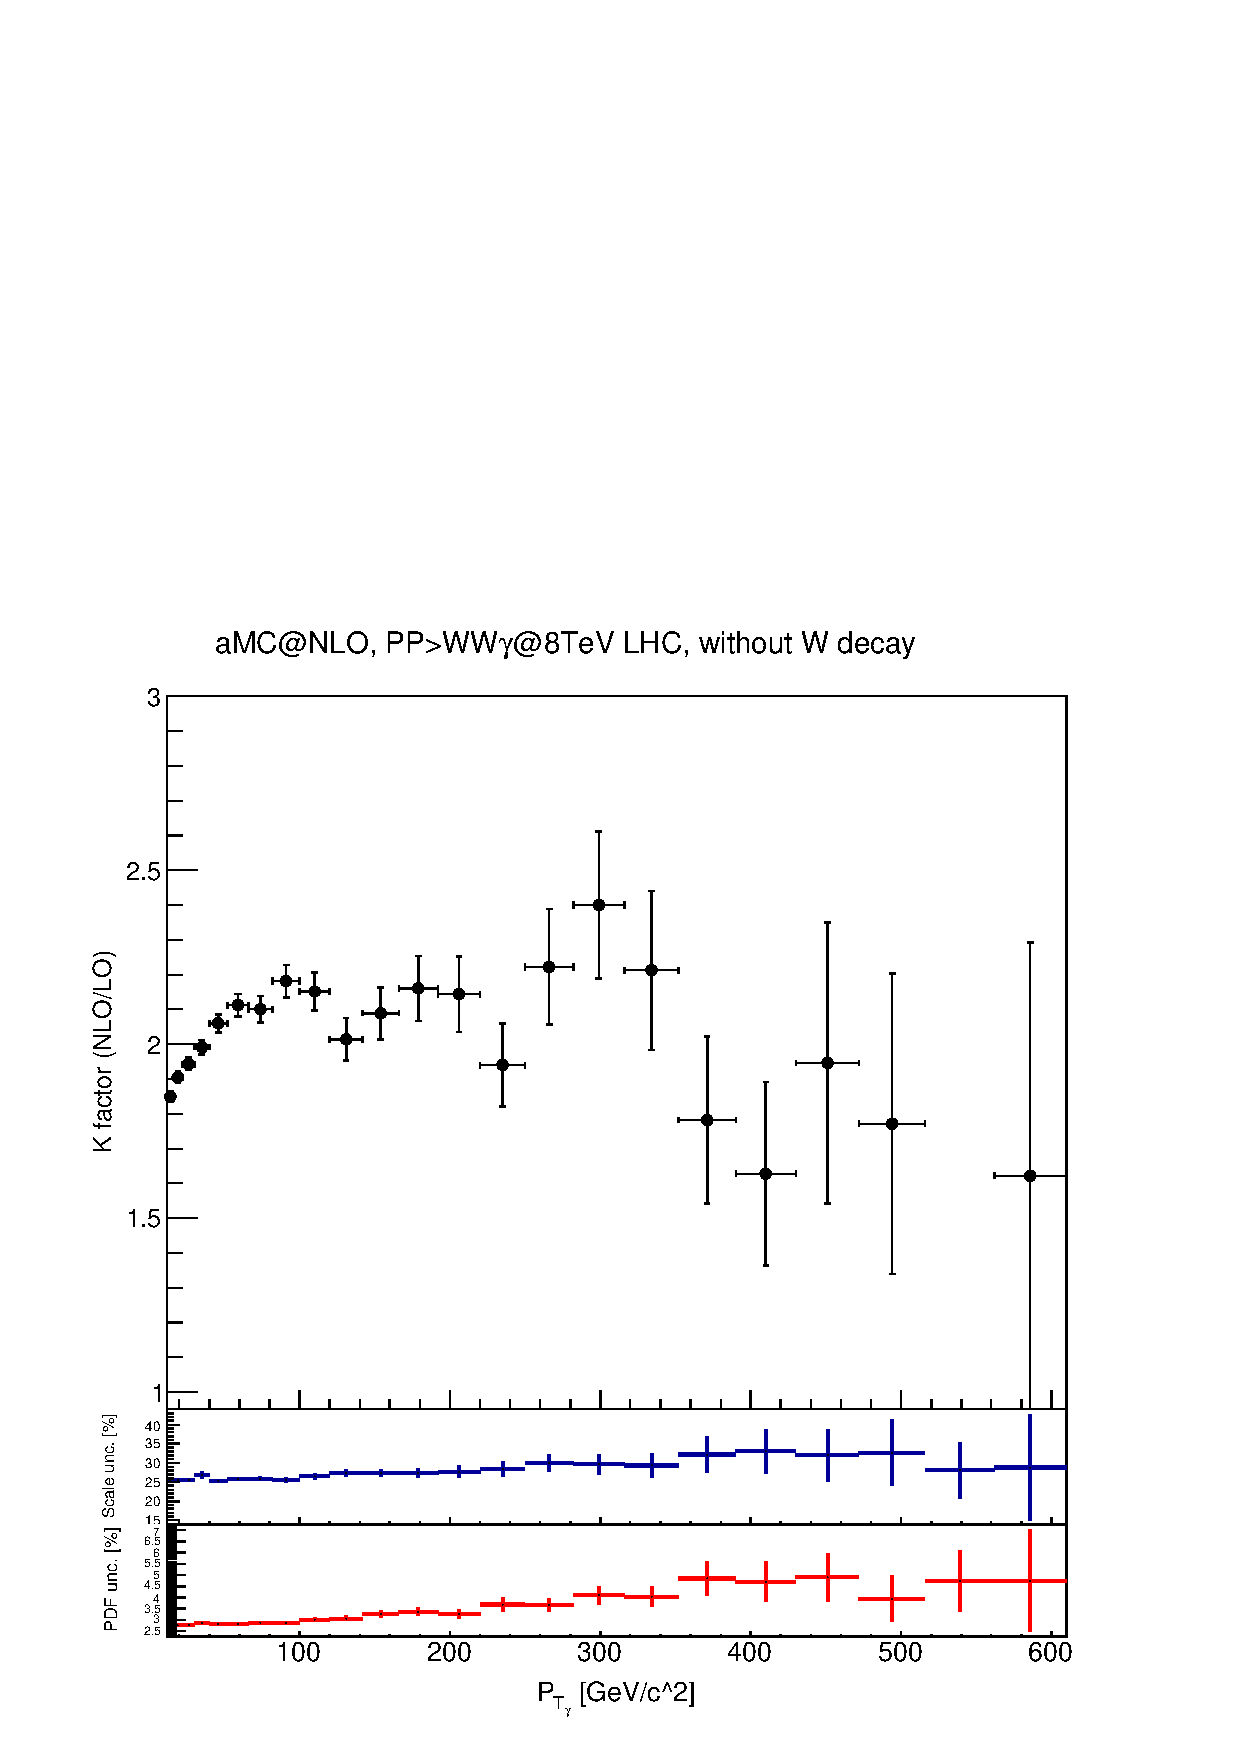
\includegraphics[width=0.4\textwidth]{figs/kwwa_pt.pdf}
\caption{\label{k-wwa} \wwa signal sample K-factor distribution as a function of $p_{T_{\gamma}}$.}}
\end{figure}

In Figure~\ref{k-wwa}, the K-factor distribution is quite flat; we use a Binned Likelihood method fit to a constant to get the value of the K-factor. 
Therefore, the K-factor value, with scale and PDF uncertainties, we use for 
the SM signal sample is 2.09812 $\pm$ 0.302029\% (stat.) $\pm$ 23.4256\% 
(scale) $\pm$ 3.55719\% (PDF).

\newpage
\subsection{aQGC K-factor}
\label{sec:aQGC_Kfac}

The MC samples for aQGC study are generated as SM WV$\gamma$ with added aQGC.
K-factor for two values of $a_{0}^{W}/\Lambda^{2}$ and $a_{C}^{W}/\Lambda^{2}$ are computed 
as function of the photon $p_{T}$ and show on Figure~\ref{k-Awwa}. At low photon $p_{T}$ the 
K-factor resembles the SM WW$\gamma$ K-factor, while with the increase of the photon $p_{T}$, most of 
the contributions are from the quardrilinear diagrams, and one can expect that the value will be similar to the Drell Yan processes.
The K-factor $p p \rightarrow W^{+}$ and $ p p \rightarrow Z$ processes have been also calculated , and the results turned out to be 
1.185 and 1.184. As can be seen in Figure~\ref{k-Awwa}, the aQGC K-factor levels at approximately 1.185 when the
photon $p_{T}$ is greater than 300 GeV/c. The exact behavior of the K-factor at low photon $p_{T}$ for the SM WW$\gamma$ with added aQGC 
depends on type of the aQGC parameter and its value. On Figure~\ref{k-Awwa} is shown the K-factor for two different aQGC parameters, 
while on Figure~\ref{k-diffvalue} is shown the K-factor for two different values of the same aQGC parameters, namely 
$a_{0}^{W}/\Lambda^{2}$.

In this study we define as visible aQGC signal only the contribution, which is originated from the anomalous quardrilinear diagrams.
The limit-setting machinery, discussed
in Section~\ref{sec:aQGClim}, uses a signal input distribution which is the
difference between the SM WV$\gamma$ with added aQGC and SM WV$\gamma$ only photon $p_{T}$ distributions (refer to as "aQGC-SM").
Since virtually all events with a photon $p_{T}$ above 300 GeV/c are predicted to
be from aQGC in our analysis, then the input distribution should reflect the
K-factor of 1.185 only. To accomplish this, when preparing the input file 
for the limit setter, we do not use a K-factor for either the SM or aQGC 
samples in the aQGC-SM subtraction. With the resulting aQGC-SM distribution
being primarily high photon $p_{T}$ events, and aQGC in nature, then we
apply the K-factor of 1.185. Since there are some remaining low photon 
$p_{T}$ aQGC events in the aQGC-SM distribution, we are applying a constant
K-factor across the board. An illustration of the resulting K-factor from such procedure is shown on Figure~\ref{k-pureaqgc}.
Photon $p_{T}$ distributions for aQGC-SM LO and NLO samples are shown on \ref{k-pureaqgc}a, while the resulting K-factor is 
shown on \ref{k-pureaqgc}b. 

\begin{figure}[]{
\centering
\includegraphics[width=0.4\textwidth]{figs/kAwwa_pt.pdf}
\caption{\label{k-Awwa} \wwa signal aQGC sample K-factor distribution as a function of $p_{T_{\gamma}}$}}
\end{figure}

\begin{figure}[]{
\centering
\includegraphics[width=0.4\textwidth]{figs/diffvalue_Kfactor.pdf}
\caption{\label{k-diffvalue} \wwa signal aQGC sample K-factor distribution with different $a_0^W/\Lambda^2$ values }}
\end{figure}

\begin{figure}[]{
\centering
\includegraphics[width=0.8\textwidth]{figs/pureaqgc_Kfactor.pdf}
\caption{\label{k-pureaqgc} \wwa signal aQGC-SM $p_{T_{\gamma}}$ distribution (left) and K factor distribution (right), with $a_0^W/\Lambda^2 = 3 \times 10^{-5} GeV^{-2}$}}
\end{figure}

As additional cross check we have calculated the K-factors for SM WV$\gamma$ with added aQGC for all values of the $a_0^W/\Lambda^2$ parameter and 
re-calculated the limits on this parameter. The limits are shown in Section~\ref{sec:aQGClim}, while the conclusion is that with either of the 
described two procedure we arrive to the same constrains on the aQGC values. Thus we have chosen to used the methods with constant Drell Yan like K-factor for 
aQGC-SM, as the precise calculation of the K-factors for all values of all studied aQGC parameter will take vary long time.
In this last cross check we have used the following function to fit the K-factor shape for SM WV$\gamma$ with added aQGC:
\begin{equation}
\begin{cases}
slp \cdot x + ( top - slp \cdot cuta), \text{     } x \leq cuta  \\
(top-1.185) \cdot exp(-tau \cdot (x-cuta)) + 1.185, \text{     } x > cuta 
\end{cases}
\label{k-fitfunc}
\end{equation}
where the slp, top, cuta, tau are fit parameters and x represent the $p_{T_{\gamma}}$. K-factors and the fit are shown on  
Figure~\ref{k-fitshape} for $a_0^W/\Lambda^2 = p \times 10^{-5} GeV^{-2}$, where $p= 2,3,5.


\begin{figure}[]{
\centering
\includegraphics[width=0.4\textwidth]{figs/a0w_kshape_p2.pdf}
\includegraphics[width=0.4\textwidth]{figs/a0w_kshape_p3.pdf}
\includegraphics[width=0.4\textwidth]{figs/a0w_kshape_p5.pdf}
%\includegraphics[width=0.4\textwidth]{figs/acw_kshape.pdf}
\caption{\label{k-fitshape} K factor shape fitted with function ~\ref{k-fitfunc}, for $a_0^W/\Lambda^2 = 2,3,5 \times 10^{-5} GeV^{-2}$  }}
\end{figure}


\subsection{W$\gamma$ + jets background estimation}

In order to estimate the normalization of the major background
W$\gamma$+jets, we used a data-driven technique.
%% The method involved analyzing sideband distributions in the W$\to$jj
%% mass spectrum in data.
%% These sidebands lie outside of a 70-100 GeV $M_{W,Z}$ window,
%% and in addition include all other normalized Monte Carlo background
%% and signal contributions, of which there was less than 0.6\% signal
%% contamination.
The background normalization in the signal region is extracted with a
binned maximum likelihood fit to the dijet invariant mass
distribution $m_{jj}$ of the two leading jets. The signal region
corresponding to the W and Z mass windows, $70 GeV < m_{jj} <
100 GeV$, is excluded from the fit.  The W$\gamma$+jets shape is
taken from simulation.  The overall normalizations of the
W$\gamma$+jets and fake photon components are allowed to vary in the
fit.  All other backgrounds, which contribute less than 10\% to the
total, are based on simulation and are fixed to their SM expectations
with uncertainties.  The multi-jet background shape is derived from
data by relaxing lepton isolation and identification requirements. Its
contribution to the total number of events is evaluated from a
separate two-component likelihood fit to the \MET
distribution, and fixed in the $m_{jj}$ fit according to this
fraction within uncertainties~(\cite{CMS-AN-12-224}, Section 11).
Normalization for the W$\gamma$+jets is measured to be $1.099 \pm
0.073$ for muons and $1.074 \pm 0.085$ for electrons. The quality of
the fit is illustrated on Figure ~\ref{fig:wapjets_kfct}

Table~\ref{tab:MCxsec} summarizes
the K-factors and cross sections used for each Monte Carlo sample,
as well as the treatment of all backgrounds in the fit.

\begin{table}[htb]
\centering
\scalebox{0.8}{
  \begin{tabular}{|l|c|c|l|}
  \hline
  MC Sample & K & $\sigma$ [pb] & External constraint on normalization \\
   &  &  & used in W$\gamma$+jets fit \\
  \hline
  \hline
  SM WW$\gamma$            & 2.1        & 0.02771    & Fixed \\
  SM WZ$\gamma$            & 2.1        & 0.00578008 & Fixed \\
  anomalous WWV$\gamma$    & 1.185      & -          & NA    \\
  W$\gamma$+jets           & 1.10(mu),1.07(el)  & 9.37246    & Unconstrained \\
  Fake photon              & from data  & -          & Constrained \\
  Multi-jet                & from data  & -          & Fixed: \MET fit in data $\pm$ 50\% (100\%) for electrons (muons) \\
  Z$\gamma$+jets           & 1          & 0.63196    & Fixed \\
  t$\overline{t}\gamma$    & 1          & 1.44       & Fixed \\
  Single Top (s-channel)   & NLO        & 3.89394    & Fixed \\
  Single Top (t-channel)   & NLO        & 55.531     & Fixed \\
  Single Top (tw-channel)  & NLO        & 11.1773    & Fixed \\
  Single Top (ps-channel)  & NLO        & 1.75776    & Fixed \\
  Single Top (pt-channel)  & NLO        & 30.0042    & Fixed \\
  Single Top (ptw-channel) & NLO        & 11.1773    & Fixed \\
  \hline
  \end{tabular}}
  \caption{List of backgrounds, the theoretical K-factors and cross
  sections used for MC-based backgrounds, and how they are treated in
  the background normalization template fit. The data-driven K-factor
  for W$\gamma$+jets sample is listed for both the muon and electron
  channels.}  \label{tab:MCxsec}
\end{table}

%% Examples of the $m_{jj}$ fit are shown in
%% Figure~\ref{fig:mjj_mH350} for the muon channel, with selections
%% optimized for Higgs mass hypotheses 190\GeVnn, 300\GeVnn, and
%% 500\GeVnn. The uncertainties in the normalization obtained from the
%% fit are propagated to the limit calculation as a systematic
%% uncertainty.  The signal $m_{jj}$ distributions are shown in
%% figure~\ref{fig:mjj_signals}.

\begin{figure}[b]
   \begin{center}
      \includegraphics[width=0.4\textwidth]{figs/mu_mjj1.pdf}
      \includegraphics[width=0.4\textwidth]{figs/el_mjj1.pdf}
      \caption{Data and MC dijet mass sidebands used to estimate the data-driven W$\gamma$+jets K-factor.}
      \label{fig:wapjets_kfct}
   \end{center}
\end{figure}



\input{DataMCcomparison}
\input{MVAselection}
%%%%%%%%%%%%%%%%%%%%%%%%%%%%%%%%%%%%%%%%%%%%%%%%%%%%%%%%%%%%%%%%%%%%%%%%%%
%%%%%%%%%%%%%%%%%%%%%%%%%%%%%%%%%%%%%%%%%%%%%%%%%%%%%%%%%%%%%%%%%%%%%%%%%%
\clearpage{}
\section{Systematic uncertainties}
\label{sec:syst}
We consider several sources of systematic uncertainty, taking into
account their effect on both the signal acceptance and on the template
shapes for the signal extraction fit.  The uncertainty on the
normalization of the backgrounds is taken as part of the statistical
uncertainty.  Other sources of
systematic uncertainty considered include jet energy scale (JES) as
well as trigger and lepton identification efficiencies.
The systematic uncertainties on signal are summarized in
Table~\ref{tab:signalSyst}.


%%%%%%%%%%%%%%%%%%%%%%%%%%%%%%%%%%%%%%%%%%%%%
%\subsection{W+jets shape}
%\label{sec:syst_wjets}
%The shape uncertainty of the W+jets template is included
%in the total fit uncertainty as described in
%Sections~\ref{sec:wjetsShape}-\ref{sec:mjj_fit}.  
%
%
%This systematics can be further analyzed by comparing the 
%fitted values of the factorization/ renormalization 
%scale (and matrix element -- parton shower matching scale)  
%in \Wev\ and \Wmv\
%events and demonstrating that the two subsets of data 
%both pick out the same scale within errors.  
%Since the physics of the W+jets should be the same while the physics
%of misidentified W bosons in multijet data can be quite different 
%in electron and muon events, this test constrains whether there 
%are background issues. 
%Table~\ref{tab:wjetsscale} lists the fraction of alternative 
%W+jets shapes (obtained by varying the factorization/ renormalization 
%and ME--PS matching scales by factors of 2) in the overall W+jets shape. 
%The values for the electron and muon data are in agreement 
%within the uncertainties.
%%%%%%%%%%%%%%%%%%%%%
%\begin{table}[bthp]
%\begin{center}
%  \begin{tabular}{l c c}
%    \hline  \hline
%     & $f_\text{scale}$ & $f_\text{ME-PS-matching}$\\
%    \hline  
%    electron  &	-0.0027 $\pm$ 0.074 & -0.136 $\pm$ 0.081\\
%    muon      &	0.053 $\pm$ 0.078 & -0.075 $\pm$ 0.065\\
%    \hline  \hline
%  \end{tabular}
%\end{center}
%\caption{\label{tab:wjetsscale} The fractions $f_\text{scale}$ and 
%$f_\text{ME-PS-matching}$ 
%(see Eq.~\ref{eqn:wjetsShapeMatchingQ2}) of the 
%W+jets process obtained from fit to electron and muon data. 
%Here $f_\text{scale}$ ($f_\text{ME-PS-matching}$) corresponds to 
%the contribution from an alternative choice of the 
%factorization/renormalization  (matrix element -- parton shower matching)
%scale. A positive fraction means that the data prefer 
%larger values for scale than in our default simulation. A negative 
%fraction means that the data prefer smaller scale. The fractions add up 
%to unity: 
%$|f_\text{scale}|$ + $|f_\text{ME-PS-matching}|$ + $f_{\text{default}}$ = 1.}
%\end{table}
%%%%%%%%%%%%%%%%%%%%%
%Figure~\ref{fig:q2NLLscan} shows the likelihood scan for the 
%factrization/renormalization and ME-PS matching scales.
%%%%%%%%%%%%%
%\begin{figure}[h!] {\centering
%    \includegraphics[width=0.48\textwidth]{figs/DibosonNLLfSU.pdf}
%    \includegraphics[width=0.48\textwidth]{figs/DibosonNLLfMU.pdf}
%    \caption{The scan of the negative log likelihood for the 
%factrization/renormalization and ME-PS matching scales. They have the 
%usual parabolic distribution with minimum near 0. The minimum values 
%correspond to the ones obtained in our nominal fit and listed in 
%Table~\ref{tab:wjetsscale}. }
%    \label{fig:q2NLLscan}}
%\end{figure}
%%%%%%%%%%%%%



%%%%%%%%%%%%%%%%%%%%%%%%%%%%%%%%%%%%%%%%%%%%
\subsection{Jet Energy Scale: AK5 Jets}
\label{sec:topw}
A dedicated analysis of 2010 data by the JetMET group showed that the jet energy
uncertainty for a generic particle-flow jet is within 3\% and the jet resolution
(JER) uncertainty is within 10\%.  For more details, see
Refs.~\cite{jetsyst,jetsyst2}.  The systematic uncertainties in the
JES and JER can affect our signal acceptance and the $m_{jj}$ distribution.
Figure~\ref{fig:ECComparison} shows a comparison of W+jets shape 
obtained using default jet energy scale with those obtained by using 
$\pm 1\sigma$ variation in the default scale.
In the present analysis, we performed several studies to cross check 
and constrain the JES/JER uncertainties. Two such studies are described 
below. We determine that the average uncertainty in the JES for the 
jet kinematics relevant to the present analysis is at the level below 1\% 
and uncertainty in JER is at the level of 10\%. These are in agreement 
with Refs.~\cite{jetsyst,jetsyst2} for jets of $p_T > 35$~\gev and 
$|\eta|<2.4$. The effect of propagating these uncertainties to the 
signal acceptance and diboson yields is minuscule. 
%%%%%%%%%%%%
%%%%%%%%%%%%
\begin{figure}[h!] {\centering
    \includegraphics[width=0.5\textwidth]{figs/JECComparison.pdf}
    \caption{Comparison of W+jets shape using default JES and 
    using $\pm 1\sigma$ variation in JES. The selection used here 
    is the same as used for muon no b-tag data.}
    \label{fig:ECComparison}}
\end{figure}
%%%%%%%%%%%%
%%%%%%%%%%%%
%%%%%%%%%%%%
%\subsubsection{Scan of jet energy scale}
%In this study we scan the JES from -5\% to +5\% and repeat the fit. 
%We performed  this test in a subset of the muon data. 
%The $\chi^2$ of the fit is plotted in
%Figure~\ref{fig:JESScanchi2} as a function of the JES shift. 
%
%The minimum in $\chi^2$ is consistent
%with the value obtained from hadronic W candidates in top
%quark events (described below) and the fit has a stable, well defined minimum. 
%Note that the above study serves a crosscheck.
%%%%%%%%%%%%%
%\begin{figure}[h!] {\centering
%    \includegraphics[width=0.5\textwidth]{figs/JES_scan.pdf}
%    \caption{$\chi^2$ of the fit vs JES shift for muon no b-tag data.}
%    \label{fig:JESScanchi2}}
%\end{figure}
%%%%%%%%%%%%

%%%%%%%%%%%%%%%%%%%%%%%%%%%%%
\subsection{Resolved Jets Control Region: $t\bar{t}$}
\label{sec:ttbar_resulved}

At LHC the top pair production rate is fairly large, almost four times larger than the diboson production
rate. According to the Standard Model, the top quark decays into $W$
boson and $b$ quark with branching fraction of about 100\%. When we
select events in which one $W$ boson decays leptonically
(\textit{i.e.}, $W\to e\nu, \mu\nu$) and the other $W$ boson decays
into quark pairs thus leading to a semileptonic final state, then the
signal purity is very high.  The final state consists of a high energy
lepton, large missing $E_T$, and four jets of which two are
$b$-tagged. The hadronic W candidates are formed from two anti-btagged
jets.  The invariant mass of the hadronic W candidates (in the muon channel) is shown in
Fig.~\ref{fig:topw:mu_MC}. As an alternative, we convolve the MC templates with a Gaussian resolution function and
repeat the fit on the control sample data (Fig.~\ref{fig:topw:mu_ConvolvedMC}). The Gaussian parameters returned by the fit are $\mu=4.28\pm 0.50$, $\sigma=3.23\pm 0.49$~GeV. They are subsequently used for convolved template fit studies presented in section~\ref{sec:convolvedMCfit}. However, the $W$ mass resolution is dominated by the resolution of the 
jet energy measurement, with JES systematics accounted for as described in section~\ref{sec:topw}.
%%%%%%%%%%%%%%%%%%%%%
%%%%%%%%%%%%%%%%%%%%%
\begin{figure}[htb] 
  {\centering
    \includegraphics[width=0.49\textwidth]{figs/topwjes/Dibosonlnujj_TopControlSample_muon_Stacked_NoConv.png}
    \includegraphics[width=0.49\textwidth]{figs/topwjes/Dibosonlnujj_TopControlSample_muon_Pull_NoConv.png}
    \caption{Template fit to the invariant mass distribution of the hadronic 
      W candidates in the muon semileptonic top sample: stacked backgrounds (left) and normalized residual between data and MC (right).}
    \label{fig:topw:mu_MC}}
\end{figure}
%%%%%%%%%%%%%%
\begin{figure}[htb] 
  {\centering
    \includegraphics[width=0.49\textwidth]{figs/topwjes/Dibosonlnujj_TopControlSample_muon_Stacked_ConvFit.png}
    \includegraphics[width=0.49\textwidth]{figs/topwjes/Dibosonlnujj_TopControlSample_muon_Pull_ConvFit.png}
    \caption{Convolved template fit to the invariant mass distribution of the hadronic 
      W candidates in the muon semileptonic top sample: stacked backgrounds (left) and normalized residual between data and MC (right).}
    \label{fig:topw:mu_ConvolvedMC}}
\end{figure}
%%%%%%%%%%%%%%
%%%%%%%%%%%%%%%%%%%%%
\subsubsection{Diboson Mass vs PU}
In addition we study the PileUp dependence of the hadronic W candidate mass in the control sample by fitting it with a Gaussian for low ($NPV<12$), medium ($12<NPV<18$) and high ($NPV>18$) PU scenarios. The results are shown in Fig.~\ref{fig:pu_TopControlSampleGausFit}; the mean and $\sigma$ values are fitted with straight lines with the resultant parameters listed in Table~\ref{tab:pu_TopControlSampleGausFit}. As expected, there is a small increase in the mean \& resolution as a function of PU, while the discrepancies between data and MC remain constant.
%%%%%%%%%%%%%%
\begin{figure}[htb] 
  {\centering
    \includegraphics[width=0.49\textwidth]{figs/puchecks/DibosonMassVsPU_mean.pdf}
    \includegraphics[width=0.49\textwidth]{figs/puchecks/DibosonMassVsPU_sigma.pdf}
    \caption{Gaussian fit results to the invariant mass distribution of the hadronic 
      W candidates in the muon semileptonic top sample for low ($NPV<12$), medium ($12<NPV<18$) and high ($NPV>18$) PU scenarios: mean (left) and $\sigma$ (right).}
    \label{fig:pu_TopControlSampleGausFit}}
\end{figure}
%%%%%%%%%%%%%%
%%%%%%%%%%%%%%%%%%%%%%%%%%
 \begin{table}[h!]
   \begin{center}
   \begin{tabular}{l|cc}
  \hline
  parameter & constant & slope \\
  \hline                                  
  $\mu_{MC}$                                  & $82.0\pm 0.2$ & $0.09\pm 0.01$ \\
  $\mu_{Data}$                                  & $83.0\pm 0.3$ & $0.08\pm0.02$ \\
  $\sigma_{MC}$                               & $12.0\pm 0.3$ & $0.08\pm 0.02$ \\
  $\sigma_{Data}$                               & $13.1\pm 0.3$ & $0.07\pm 0.02$ \\
  \hline
   \end{tabular}
   \end{center}
   \caption{Linear dependence of the mean and resolution of the gaussian fit to the invariant mass distribution of the hadronic 
      W candidates in the muon semileptonic top sample. The increase as a function of $NPV$ is statistically consistent between MC and Data.} 
   \label{tab:pu_TopControlSampleGausFit}
 \end{table}
%%%%%%%%%%%%%%%%%%%%%%%%%

%%%%%%%%%%%%%%%%%%%%%%%%%%%%%
%--------------------------------------------------
\subsection{Jet Energy Scale: CA8 Jets}
\label{sec:systematicsCA8}
The CA8 jets are corrected using the AK7 dedicated corrections.  
The systematic uncertainty is estimated by varying up and down the jet energy uncertainties and computing the effect on the mean jet mass in the 
$t\bar{t}$ control sample.  

Additional uncertainties are added in quadrature to the AK7 jet uncertainties in order to account for the CA8 jets.  
In order to compute this additional uncertainty, we take signal MC samples and match AK7 jets to CA8 jets and 
take the fractional difference between them as an additional uncertainty. 
The matching is done for AK7 and CA8 collections for events passing preselection criteria and are matched with $\Delta R < 0.3$ criteria.
The fractional difference is computed as a function of $p_T$ and $\eta$ and is fit with a Gaussian.
In the top left and right of Fig.~\ref{fig:CA8vAK7}, we show the fitted mean and sigma fractional difference between the matched AK7 and CA8 jets 
as a function of jet $\eta$.
In the bottom left and right of Fig.~\ref{fig:CA8vAK7}, we show the fitted mean and sigma fractional difference between the matched AK7 and CA8 jets 
as a function of jet $p_T$.

\begin{figure}[htbp]
\centering
\includegraphics[width=0.48\textwidth]{figs/diff_CA8vAK7_vEta_mean}
\includegraphics[width=0.48\textwidth]{figs/diff_CA8vAK7_vEta_sigma}\\
\includegraphics[width=0.48\textwidth]{figs/diff_CA8vAK7_vPt_mean}
\includegraphics[width=0.48\textwidth]{figs/diff_CA8vAK7_vPt_sigma}\\
\caption{Fitted mean and sigma fractional difference between the matched AK7 and CA8 jet $p_T$ as a function of jet $\eta$ (top) and $p_T$ (bottom).}
\label{fig:CA8vAK7}
\end{figure}

From the plots in Fig.~\ref{fig:CA8vAK7}, we find that an additional 2\% uncertainty on the jet energy scale uncertainty added in quadrature
with the computed AK7 corrections are enough to cover scale differences due to not having dedicated corrections for CA8 jets.

%%%%%%%%%%%%%%%%%%%%%%%%%%%%%
\subsection{Merged Jets Control Region: $t\bar{t}$}
\label{sec:ttbar_merged}

To understand the performance of merged W bosons, we use a control sample of pure W's in the data from the high pT $t\bar{t}$ sample. Namely, we use the standard kinematic preselection cuts described above, but invert the cut on the number of b-tagged AK5 jets outside of the CA8 jet requiring that there is at least one CSV "medium" AK5 b-jet.
To boost statistics, we choose the CA8 jet in the opposite hemisphere of the lepton with the highest mass and a pT $>$ 200 GeV.
This is contrary to the standard selection which uses the high pT CA8 jet in the event with a pT $>$ 200 GeV.

Furthermore, for the $WW/WZ$ and signal contributions, we are concerned with the data/MC scale factor for the {\it pure} W-jet
tagging efficiency.  
In order to understand the part of the $t\bar{t}$ jet mass distribution which contains "real" merged W's and pure combinatorial background
we use the $t\bar{t}$ MC sample. 
By matching the CA8 jet with the hadronic $W$ at generator level in a cone of $\Delta R < 0.3$, we can get expected shapes.  
These plots are shown in Fig.~\ref{fig:genMatchTTbar} before and after a cut on $\tau_2/\tau_1<0.55$.  
The functional forms we choose are $f_{bkg}(x) = {\rm Exp}*{\rm Erf}$ for the unmatched sample and $f_{sig}(x) = {\rm Gaus1} + {\rm Gaus2}$ for the matched sample.

\begin{figure}[htbp]
\centering
\includegraphics[width=0.48\textwidth]{figs/topwjes/GEN_all_nocut.pdf}
\includegraphics[width=0.48\textwidth]{figs/topwjes/GEN_all_cutT2T1.pdf}
\caption{Matched and unmatched samples of $t\bar{t}$ MC sample in $t\bar{t}$ control region before (left)
and after (right) the cut of $\tau_2/\tau_1<0.55$.}
\label{fig:genMatchTTbar}
\end{figure}

We then extract the scale factors by first estimating the cut efficiency on both data and MC.
This gives us simultaneously "pass" and "fail" samples where we can then simultaneously fit to get the cut efficiency.  
The difference in the data and MC efficiencies are taken as the W-tagging efficiency.
The fit results are shown in Fig.~\ref{fig:ttbarControl_nocut}.
The fitting functions are motivated by the shapes in Fig.~\ref{fig:genMatchTTbar}.
The scale factor for electrons and muons are computed to be 0.997 and 0.993, respectively where the uncertainty on the scale factor is 7.5\%.
These scale factors are applied to the $WW/WZ$ and signal contributions.  

To extract the jet mass scale uncertainty and resolution scale factor, we fit the mass peak in the signal region.  
%The $t\bar{t}$ control sample is fit with a functional form $f(x) = {\rm Exp}*{\rm Erf} + {\rm Gaus1}*{\rm Gaus2}$.
The fits are shown for the medium $W$-tag cut in the right side plots of Fig.~\ref{fig:ttbarControl_nocut}.
The fit means and sigma of the core Gaussian in the muon channel is found to be:
\begin{eqnarray}
\langle m \rangle_{\rm MC} = 83.3 \pm 0.5~{\rm GeV}{\rm {~,~}}\sigma_{\rm MC} = 7.1 \pm 0.3~{\rm GeV} \\
\langle m \rangle_{\rm data} = 83.7 \pm 0.5~{\rm GeV}{\rm {~,~}}\sigma_{\rm MC} = 7.7 \pm 0.4~{\rm GeV} 
\end{eqnarray}

The fit means and sigma of the core Gaussian in the electron channel is found to be:
\begin{eqnarray}
\langle m \rangle_{\rm MC} = 83.3 \pm 0.6~{\rm GeV}{\rm {~,~}}\sigma_{\rm MC} = 6.7 \pm 0.4~{\rm GeV} \\
\langle m \rangle_{\rm data} = 83.9 \pm 0.6~{\rm GeV}{\rm {~,~}}\sigma_{\rm MC} = 7.9 \pm 0.5~{\rm GeV}
\end{eqnarray}
We find that the mass scale systematic is unity to within errors but that the W-jet resolution is larger in the data.
Since we do not expect that the resolution should differ between electron and muon channels, we average the difference as 
$\bar{\sigma}_{MC}$  = 7.0 and $\bar{\sigma}_{data}$  = 7.8. 
We correct the MC resolution by 11\% to correct for the difference in data/MC.

\begin{figure}[htbp]
\centering
\includegraphics[width=0.45\textwidth]{figs/topwjes/control_medium_el_without_tau2tau1.pdf}
\includegraphics[width=0.45\textwidth]{figs/topwjes/control_medium_el_with_tau2tau1.pdf}\\
\includegraphics[width=0.45\textwidth]{figs/topwjes/control_medium_mu_without_tau2tau1.pdf}
\includegraphics[width=0.45\textwidth]{figs/topwjes/control_medium_mu_with_tau2tau1.pdf}\\
\caption{Pruned jet mass distribution in the $t\bar{t}$ control sample before (left) and after (right) applying $\tau_2/\tau_1<0.55$ cut.}
\label{fig:ttbarControl_nocut}
\end{figure}
%%%%%%%%%%%%%%%%%%%%%%%%%%%%%

%--------------------------------------------------
\subsection{Lepton selection and trigger efficiency}
\label{sec:LeptonSelectionAndTriggerEfficiency}
%%The lepton trigger and selection is common among several CMS analyses and 
%%we benefit from common studies based on tag-and-probe techniques. 
%%
Systematic uncertainties in the trigger efficiencies in
Section~\ref{sec:Eff} are of the order of 1\%. Systematic
uncertainties in the lepton reconstruction and identification
efficiency scale factors are of the order of 2\%. These uncertainties
are accounted for in the final systematics that are input to the
cross-section uncertainty calculation.
%--------------------------------------------------
\subsection{MET uncertainty}
MET directly affects our signal acceptance. 
The uncertainty prescription is discussed in Ref.~\cite{met}.
%https://twiki.cern.ch/twiki/bin/viewauth/CMS/MissingETUncertaintyPrescription
In addition, the MET distribution in the data is $\simeq$3\% wider 
than the MC, and placing a hard MET$>30.0$ cut creates an uncertainty. 
We estimate it by smearing the MET for each event by a Gaussian with 
a $\sigma =0.03*$MET and observing how many events pass the cut. 
Specifically, (Events Passing After Smearing)/(Events Passing Before Smearing) 
=0.998 for both muons and electrons.
%%%%%%%%%%%%%%%%%%%%%%%%%%%%
\subsection{Cross-section of nuisance backgrounds}
The uncertainties in the cross sections of other backgrounds 
like $\ttbar$,  single top, QCD multi-jets, and Z+jets processes 
are already propagated by letting their normalization (i.e., yield) 
float in the fit within a constraint.

%%%%%%%%%%%%%%%%%%%%%%%%%%%%%
\subsection{Theory uncertainty in acceptance}
The theory uncertainty on the signal acceptance due to variations in the parton distribution functions and the
value of $\alpha_{s}$ is obtained by following the {\sc pdf4lhc} prescription ~\cite{Botje:2011sn}.
Using \textsc{CT10}~\cite{ct10}, \textsc{MSTW08}~\cite{Martin:2009iq}, and \textsc{NNPDF}~\cite{nnpdf} sets, the uncertainties are estimated to be 2.3\% 
for $q\bar{q} \to WW$ and and 0.8\% for $gg \to WW$ by the leptonic $WW$ group (SMP-12-024).
Likewise, the impact of higher-order corrections is estimated by varying the QCD renormalisation
($\mu_R$) and factorization ($\mu_F$) scales up and down by a factor of two using the \textsc{mcfm} program~\cite{MCFMarticle} and found to be 1.5\%. 
The overall theory uncertainty is below 3\%, consistent with our studies at 7~TeV (AN-12-224).



%For the 7TeV analysis we compute theory uncertainty in acceptance for muon ``no b-tag'' selection 
%using MCFM: $\pt^{\text{jet}}>35$~GeV, $|\eta^{\text{jet}}|<2.4$, 
%$\pt^{\text{lepton}}>325$~GeV, $|\eta^{\text{lepton}}|<2.1$, 
%$\met > 30$~GeV, W $m_T > 30$~GeV, $\Delta{R}$ (lepton, jet) $>0.3$, 
%no additional lepton. 
%We use CTEQ6.6m as the default PDF and the quantity $\mu_0 = \sqrt{M_W^2 + p_{T, W}^2}$ as  
%the default factorization/renormalization scale.
%For systematic studies 
%we vary the choices of PDF and the factorization/renormalization 
%scale. The details are shown in Table~\ref{tab:theorysyst}. 
%The overall theory 
%uncertainty is below 3\%.
% %%%%%%%%%%%%%%%%%%%%%%%%%%%
% \begin{table}[h!]
%   \begin{center}
%   \begin{tabular}{l|c}
%  \hline
%  \hline
%  Source of uncertainty & Relative variation in acceptance value \\
%  \hline                                  
%  PDF: CT10                             & $1.4\%$ \\
%  PDF: CTEQ61M                          & $-0.7\%$ \\
%  PDF: MSTW8NL                          & $0.4\%$ \\
%  PDF: MSTW8NN                          & $0.1\%$ \\
%  PDF: MSTW8LO                          & $-1.3\%$ \\
%  Scale: $2~\mu_0$                      & $-0.01\%$ \\
%  Scale: $0.5~\mu_0$                    & $0.8\%$ \\
%  Scale: $\sqrt{M_W^2 + p_{T, jet1}^2}$ & $-0.3\%$ \\
%  Scale: $H_T$                          & $0.1\%$ \\
%  \hline
%  \hline
%   \end{tabular}
%   \end{center}
%   \caption{Theory uncertainty in acceptance. The central value for 
%   acceptance $\times$ branching fraction is $(1.279 \pm 0.019) \times 10^{-2}$.} 
%   \label{tab:theorysyst}
% \end{table}
% %%%%%%%%%%%%%%%%%%%%%%%%%
%%%%%%%%%%%%%%%%%%%%%%%%%%%%
\subsection{Uncertainty in jet veto efficiency}
Since we use events with exactly two jets, we reject signal events 
which have extra jet(s) from ISR or FSR. Our acceptance computation 
takes this inefficiency into account. However, there is a 
systematic uncertainty associated with the modeling of 
ISR/FSR in our simulation. The effect has been studied by the WW group and is expected to be less than 5\% (SMP-12-024).

%For the 7TeV analysis, to estimate this systematics we 
%compare the efficiency of our jet veto at generator-level 
%(i.e., using ``GenJets'') in the Pythia WW, Pythia WZ, and 
%privately produced MadGraph WW samples. All three simulations 
%use LO matrix element calculation, parton showering from 
%Pythia, and identical choices of factorization/renormalization
%scales and PDFs. However, the soft gluon radiation probability 
%is different in each sample.  
%Table~\ref{tab:jetvetoeff} lists the jet-veto efficiency 
%in each of the three samples. We take the maximum 
%difference in efficiency as a systematic uncertainty.
%This systematic is within 2\%.
%%%%%%%%%%%%%%%%%%%%%%%%%%%
% \begin{table}[h!]
%   \begin{center}
%   \begin{tabular}{l|c}
%  \hline
%  \hline
%  Sample & jet-veto efficiency \\
%  \hline                                  
%  WW Pythia                             & $88.72\%$ \\
%  WZ Pythia                             & $87.48\%$ \\
%  WW MadGraph                           & $89.57\%$ \\
%  \hline
%  \hline
%   \end{tabular}
%   \end{center}
%   \caption{Jet-veto efficiency in various diboson simulations.} 
%   \label{tab:jetvetoeff}
% \end{table}
%%%%%%%%%%%%%%%%%%%%%%%%%%
%%%%%%%%%%%%%%%%%%%%%%%%%%%%
\subsection{Luminosity uncertainty}
\label{sec:LumiUncertainty}
The latest recommendation for the uncertainty on LHC luminosity is 2.6$\%$~\cite{lumiPAS}.
We propagate this uncertainty to the expected yield of the signal and from there to the
calculated cross-section.
%%%%%%%%%%%%%%%%%%%%%%%%%%%%
%%%%%%%%%%%%%%%%%%%%%%%%%
 \begin{table}[h!]
   \begin{center}
   \begin{tabular}{l|c}
  \hline
  \hline
  Source of uncertainty & Magnitude \\
  \hline                                  
  Luminosity                             & 2.6\%$ \\
  \hline 
  Jet energy scale, resolution, and \MET & $<1\%$ \\
  Theory acceptances (PDF)               & $<3\%$ \\
  ISR/FSR acceptances                    & $<5\%$ \\
  Lepton trigger eff.                    & $1\%$ \\
  Lepton selection eff.                  & $2\%$ \\
  Pile-up                                & $<1\%$ \\
  b-tag veto                             & $<1\%$  \\
  \hline 
  total (without Luminosity)             & $<6.5\%$  \\
  \hline
  \hline
   \end{tabular}
   \end{center}
   \caption{Sources of signal systematics considered in the analysis, with the corresponding magnitude.} 
   \label{tab:signalSyst}
 \end{table}
%%%%%%%%%%%%%%%%%%%%%%%%%

%%%%%%%%%%%%%%%%%%%%%%%%%%%%%%%%%%%%%%%%%%%%%%%%%%%%%%%%%%%%%%%%%%%%%%%%%%
%%%%%%%%%%%%%%%%%%%%%%%%%%%%%%%%%%%%%%%%%%%%%%%%%%%%%%%%%%%%%%%%%%%%%%%%%%
\clearpage{}
\section{WW$\gamma$/WZ$\gamma$ cross section measurement}
\label{sec:sys}
% ---- ---- ---- ---- ---- ---- ---- ---- ---- ---- ---- ---- ---- ---- ----
%A measurement of the WW$\gamma$/WZ$\gamma$ cross section is derived using
%
%\begin{center}
%\begin{equation}
%   \sigma = \frac{N_{data}-N_{bkg}}{L \cdot A \cdot \varepsilon_{MC} \cdot SF}
%\label{eq:xsection}
%\end{equation}
%\end{center}
%
%where $\sigma$ is the measured cross section, $N_{data}$ is the number of
%selected events observed in data, $N_{bkg}$ is the number of selected 
%background events predicted from Monte Carlo, L is the integrated 
%luminosity, A is the signal acceptance predicted from Monte Carlo, 
%$\varepsilon_{MC}$ is the Monte Carlo event selection efficiency, and SF 
%is the efficiency scale factor between data and Monte Carlo 
%($\frac{\varepsilon_{data}}{\varepsilon_{MC}}$), such as those listed for
%the photon in Table~\ref{tab:photon_eff}.  Each of these values has an 
%associated systematic and statistical error that must be propagated 
%through equation~\ref{eq:xsection}.  Using standard error propagation, 
%the uncertainty in the cross sectional measurement is derived using
%
%\begin{center}
%\begin{equation}
%  \delta\sigma = |\sigma|\sqrt{(\frac{{\delta}N_{sig}}{N_{sig}})^{2}+(\frac{{\delta}L}{L})^{2}+(\frac{{\delta}A}{A})^{2}+(\frac{\delta\varepsilon_{MC}}{\varepsilon_{MC}})^{2}+(\frac{{\delta}SF}{SF})^{2}}
%\label{eq:xsec_unc}
%\end{equation}
%\end{center}

%where $N_{sig}$ = $N_{data}-N_{bkg}$ and thus

%\begin{center}
%\begin{equation}
%   {\delta}N_{sig} = \sqrt{({\delta}N_{data})^{2}+({\delta}N_{bkg})^{2}}.
%\end{equation}
%\end{center}

%With equations~\ref{eq:xsection} and \ref{eq:xsec_unc}, Table~\ref{tab:xsec_num} lists the values used to measure the WW$\gamma$ cross section.

%\begin{table}[htb]
%\centering
%\scalebox{0.70}{
%  \begin{tabular}{|c|c|c|c|}
%  \hline
%  Variable & Value & Systematic Uncertainty & Statistical Uncertainty \\
%  \hline
%  \hline
%  $N_{data}$                          & 98.0 & ----   & 9.9   \\
%  $N_{bkg}$                           & 112.6 & 9.7   & 4.7   \\
%  L                                   & 19.3  & ----   & 0.6    \\
%  A $\cdot \varepsilon_{MC} \cdot$ SF & 0.004 & 0.0002 & 0.0002 \\
%  \hline
%  \end{tabular}}
%  \caption{List of values and uncertainties used in measuring the WW$\gamma$ cross section.}
%  \label{tab:xsec_num}
%\end{table}

%Using the values in Table~\ref{tab:xsec_num}, the measured cross section for WW$\gamma$ is $\sigma$ = -168.4 $\pm$ 112.9 (Sys.) $\pm$ 127.0 (Stat.) fb.  This measurement takes into account the K-factors used for WW$\gamma$/WZ$\gamma$ and W$\gamma$+Jets processes listed in Section~\ref{sec:Kfact}, as well as the MVA discussed in Section~\ref{sec:MVA}.  The theoretical cross section provided by MadGraph 5 for semileptonic WW$\gamma$ is 41 fb, again taking into account the K-factor for WW$\gamma$ listed in Section~\ref{sec:Kfact}~\cite{MadGraph}.

This SM cross sectional measurement's uncertainties are large due to the low signal 
statistics, the uncertainties in the K-factors used, and the fake photon 
rate's systematic uncertainty of 12-39\%; therefore, we cannot claim an 
observation of WW$\gamma$ events.

The Standard Model WW$\gamma$/WZ$\gamma$ signal strength with and without
MVA optimization is shown in Figure~\ref{fig:signalstrength}, with the 
1-$\sigma$ and 2-$\sigma$ bands. Figure~\ref{fig:signalstrength} 
demonstrates that a signal strength below 1 suggests we are sensitive to 
the signal and can measure the cross section; however, we are well above 
a value of 1 and are therefore not sensitive to the SM signal. It can be 
seen that MVA optimization makes a small improvement on our sensitivity,
and optimizes our sensitivity at a MVA cut of 0.2. 
While the MVA selection helps to improve sensitivity of the measurement it is not changing the fact that only a upper cross section limit is derived for $WV\gamma$. 
Thus we consider the $WV\gamma$ upper cross section limit without use of MVA as the primary result and keep the study documented for future iterations of the analysis.

\begin{figure}[h]
  \begin{center}
    \includegraphics[width=0.75\textwidth]{figs/WVAsignalstrength.pdf}
    \caption{Standard Model WW$\gamma$/WZ$\gamma$ signal strength with various MVA cut values. A strength at or below 1 suggests we are sensitive to the SM signal.}
    \label{fig:signalstrength}
  \end{center}
\end{figure}



%%%%%%%%%%%%%%%%%%%%%%%%%%%%%%%%%%%%%%%%%%%%%%%%%%%%%%%%%%%%%%%%%%%%%%%%%%
%%%%%%%%%%%%%%%%%%%%%%%%%%%%%%%%%%%%%%%%%%%%%%%%%%%%%%%%%%%%%%%%%%%%%%%%%%
\clearpage{}
\section{AQGC parametrization and limits}
\label{sec:aQGClim}
% ---- ---- ---- ---- ---- ---- ---- ---- ---- ---- ---- ---- ---- ---- ----

\subsection{Parametrizations}
In order to set limits on anomalous couplings, we compare the observed 
signal data's kinematics to those of anomalous signal Monte Carlo.  This 
process can involve generating many different Monte Carlo samples for 
various values of each anomalous quartic coupling parameter, or we could 
quantize how anomalous couplings affect certain observable kinematical 
distributions such as photon $p_{T}$ or WW$\gamma$ invariant mass.  

In order to quantize the affect each coupling parameter has on a kinematical
distribution, say photon $p_{T}$, we still generate a few Monte Carlo 
samples for each anomalous coupling parameter, where the parameter of 
interest is varied to multiple values and all other coupling parameters set 
to their standard model value.  For example, we have five quadratic coupling
parameters $\frac{a_{0}^{W}}{\Lambda^{2}}, \frac{a_{C}^{W}}{\Lambda^{2}}, 
\frac{f_{T,0}}{\Lambda^{4}}, \frac{\kappa_{0}^{W}}{\Lambda^{2}}$, and 
$\frac{\kappa_{C}^{W}}{\Lambda^{2}}$.  In 
order to parametrize the affect the parameter 
$\frac{a_{0}^{W}}{\Lambda^{2}}$ has on photon $p_{T}$, we vary this 
parameter's values while fixing $\frac{a_{C}^{W}}{\Lambda^{2}}, 
\frac{f_{T,0}}{\Lambda^{4}}, \frac{\kappa_{0}^{W}}{\Lambda^{2}}, $and$ 
\frac{\kappa_{C}^{W}}{\Lambda^{2}}$ to their
Standard Model values of zero.

In addition to the Standard Model sample, we generate six Monte Carlo AQGC 
samples for variation in each parameter.  Then, after applying event 
selection cuts described in sections~\ref{sec:evtSel} and~\ref{sec:photon}, 
efficiency and pileup weights, and the photon $p_{T}$-dependent k-factor 
described in section~\ref{sec:Kfact}, each sample's photon $p_{T}$ 
distribution is divided by the standard model photon $p_{T}$ distribution to
form a AQGC/SM ratio for each photon $p_{T}$ bin. A quadratic distibution is
formed by plotting each AQGC/SM ratio value for a specific photon $p_{T}$ 
bin, as can be seen in Figure~\ref{fig:para_ptbins} for 
$\frac{a_{0}^{W}}{\Lambda^{2}}$ in the muon channel. 
Figure~\ref{fig:para_ptbins}-(a) exhibits a quadratic fit that decreases
with increasing AQGC: (1) this is only found to happen with $a_{0}^{W}$
and with this binning and (2) it is allowed because the limits for this
parameter fall within the fit's range and thus we benefit from minimizing
$\chi^{2}$.

\begin{figure}[]
  \begin{center}
    \subfigure[]{
    \includegraphics[width=0.33\textwidth]{figs/a0W_PhotonPT_para_bin1.png}
  }
    \subfigure[]{
    \includegraphics[width=0.33\textwidth]{figs/a0W_PhotonPT_para_bin2.png}
  }
    \subfigure[]{
    \includegraphics[width=0.33\textwidth]{figs/a0W_PhotonPT_para_bin3.png}
  }\\
    \subfigure[]{
    \includegraphics[width=0.33\textwidth]{figs/a0W_PhotonPT_para_bin4.png}
  }
    \subfigure[]{
    \includegraphics[width=0.33\textwidth]{figs/a0W_PhotonPT_para_bin5.png}
  }
    \subfigure[]{
    \includegraphics[width=0.33\textwidth]{figs/a0W_PhotonPT_para_bin6.png}
  }\\
    \subfigure[]{
    \includegraphics[width=0.33\textwidth]{figs/a0W_PhotonPT_para_bin7.png}
  }
    \subfigure[]{
    \includegraphics[width=0.33\textwidth]{figs/a0W_PhotonPT_para_bin8.png}
  }
    \subfigure[]{
    \includegraphics[width=0.33\textwidth]{figs/a0W_PhotonPT_para_bin9.png}
  }\\
    \subfigure[]{
    \includegraphics[width=0.33\textwidth]{figs/a0W_PhotonPT_para_bin10.png}
  }
    \caption{AQGC/SM ratio values for each $a_{0}^{W}/\Lambda^{2}$ Monte Carlo sample (muon channel) within each of the following Photon $p_{T}$ bins: Photon $p_{T}$ bins (a) 30-72 GeV, (b) 72-114 GeV, (c) 114-156 GeV, (d) 156-198 GeV, (e) 198-240 GeV, (f) 240-282 Gev, (g) 282-324 GeV, (h) 324-366 GeV, (i) 366-408 GeV, 408-inf. GeV (overflow bin)}
  \label{fig:para_ptbins}
  \end{center}
\end{figure}

We fit this quadratic distribution with a quadratic function that can later 
be used to predict the AQGC/SM ratio value for any arbitrary anomalous 
coupling value for that specific coupling parameter and photon $p_{T}$ bin. 
It can even been seen in Figure~\ref{fig:para_ptbins} that the overflow 
photon $p_{T}$ bin has a quadratic behavior in AQGC and thus can be 
parametrized.  

Keeping in mind that the AQGC/SM ratio fit function for a given coupling 
parameter is a function of the coupling parameter's value and depends on the
photon $p_{T}$ bin, we then plot and fit the coefficients of the AQGC/SM 
quadratic fit function versus photon $p_{T}$ in order to obtain the 
$p_T{}$-dependence of the AQGC/SM ratio.  Therefore, we obtain a 
parametrization of the affect each anomalous coupling parameter has on 
photon $p_{T}$ by substituting the $p_{T}$-dependent coefficient fit 
functions into the coupling parameter-dependent AQGC/SM ratio fit function, 
as shown in equation~\ref{parameq}.

\begin{center}
\begin{equation}
R(parameter,p_{T}) = \frac{\# AQGC events(parameter,p_{T})}{\# SM events(p_{T})} = 1 + C_{0}(p_{T}) \cdot parameter + C_{1}(p_{T}) \cdot parameter^{2}
\label{parameq}
\end{equation}
\end{center}

A closure test can be performed using equation~\ref{parameq} as a 
reweighting function applied to the Standard Model photon $p_{T}$ spectrum, 
as can be seen in Figure~\ref{fig:para_closure} for 
$\frac{a_{0}^{W}}{\Lambda^{2}}$ where the simulated (parametrized) Monte 
Carlo is compared to the generated (true) Monte Carlo.  Furthermore, the 
ratio between some of the simulated and generated Monte Carlo of each AQGC 
parameter can be seen in Figure~\ref{fig:para_closure_ratio}, where the 
deviation in each photon $p_{T}$ bin remains below 40\%.  The deviation in 
the overflow photon $p_{T}$ bin for each AQGC parameter remains below 15\% 
as well. A closure test ratio plot is also included in
Figure~\ref{fig:para_closure_ratio} for $\frac{a_{0}^{W}}{\Lambda^{2}}$ when using
a form factor of $\Lambda = 500 GeV, n = 2$.

\begin{figure}[]
  \begin{center}
    \subfigure[]{
    \includegraphics[width=0.45\textwidth]{figs/a0W_p5_closure.png}
  }
    \subfigure[]{
    \includegraphics[width=0.45\textwidth]{figs/a0W_m5_closure.png}
  }
    \caption{Photon $p_{T}$ of simulated (Red line) and generated (Blue line) Monte Carlo samples for (a) $a_{0}^{W}/\Lambda^{2}$ = 5E-05 $GeV^{-2}$ and (b) $a_{0}^{W}/\Lambda^{2}$ = -5E-05 $GeV^{-2}$ (both are muon channel)}
  \label{fig:para_closure}
  \end{center}
\end{figure}

\begin{figure}[]
  \begin{center}
    \subfigure[]{
    \includegraphics[width=0.45\textwidth]{figs/a0W_ratio.png}
  }
    \subfigure[]{
    \includegraphics[width=0.45\textwidth]{figs/acW_ratio.png}
  }\\
    \subfigure[]{
    \includegraphics[width=0.45\textwidth]{figs/lt0_ratio.png}
  }
    \subfigure[]{
    \includegraphics[width=0.45\textwidth]{figs/aQGC_K0W_closure_ratio.png}
  }\\
    \subfigure[]{
    \includegraphics[width=0.45\textwidth]{figs/aQGC_KCW_closure_ratio.png}
  }
    \subfigure[]{
    \includegraphics[width=0.45\textwidth]{figs/a0W_500FFn2_ratio.png}
  }
    \caption{Muon channel Simulated:Generated ratio as a function of photon $p_{T}$ for (a) $a_{0}^{W}/\Lambda^{2}$ = -5E-05 $GeV^{-2}$ (Red line), 5E-05 $GeV^{-2}$ (Blue line); (b) $a_{C}^{W}/\Lambda^{2}$ = -8E-05 $GeV^{-2}$ (Red line), 8E-05 $GeV^{-2}$ (Blue line); (c) $f_{T,0}/\Lambda^{4}$ = -8E-11 $GeV^{-2}$ (Red line), 8E-11 $GeV^{-2}$ (Blue line); (d) $\kappa_{0}^{W}/\Lambda^{2}$ = -2E-5 $GeV^{-2}$ (Red line), 2E-5 $GeV^{2}$ (Blue line); (e) $\kappa_{C}^{W}/\Lambda^{2}$ = -3E-5 $GeV^{-2}$ (Red line), 3E-5 $GeV^{2}$ (Blue line); (f) $a_{0}^{W}/\Lambda^{2}$ = -140E-05 $GeV^{-2}$ (Red line), 140E-05 $GeV^{-2}$ (Blue line) incorporating a Form Factor of $\Lambda = 500 GeV, n = 2$.}
  \label{fig:para_closure_ratio}
  \end{center}
\end{figure}

\newpage
\subsection{Limits using Photon $p_{T}$}
\label{sec:limits_pT}
We use the photon $p_T$ distribution as observable to set limit on anomalous
couplings.

We use the ``Higgs Combination'' package \cite{cite:combine} for
setting exclusion limits. This package is a
RooStats\cite{cite:roostats}-based statistical analysis tool-set
recommended by the CMS Higgs PAG and approved by CMS statistics committee.

We take as inputs the photon $p_T$ distributions for each signal model 
(\textit{i.e.}, various choices of $a_{0}^{W}/\Lambda^{2}$,  
$a_{C}^{W}/\Lambda^{2}$, $f_{T,0}/\Lambda^{4}$, $\kappa_{0}^{W}/\Lambda^{2}$, and 
$\kappa_{C}^{W}/\Lambda^{2}$), data, and total background that survive after
analysis cuts. All of these distributions are segregated by lepton flavor,
which represent independent channel inputs to the limit setter. 
Figure~\ref{fig:limitinput} shows the muon channel for given values of AQGC 
parameters, with and without MVA optimization (cut at 0.5), in which the AQGC input is the 
excess events from the SM prediction. For the MVA case in Figure~\ref{fig:limitinput},
the $f_{T,0}/\Lambda^{4}$ sample had diminished statistics after the cut on the MVA output
was made. We supply these distributions over the 
range $30-450~\GeV/c$ in the form of histograms to the limit setter. The binning 
is chosen such that the left-most bin begins at the first 2012 dataset point, and the 
right-most bin begins just beyond the last 2012 dataset point. We extend the
right-most bin to be an overflow bin, and since it begins just beyond the
reach of 2012 data in our events, it represents physics beyond our
sensitivity.

\begin{figure}[b]
  \begin{center}
    \subfigure[]{
      \includegraphics[width=0.45\textwidth]{figs/mu_limit_input.pdf}
    }
    \subfigure[]{
      \includegraphics[width=0.45\textwidth]{figs/mu_limit_input_MVA.pdf}
    }
    \caption{ Input photon $p_{T}$ distributions for the limit setter of the muon channel (a) without MVA optimization and (b) with MVA optimization, cut at 0.5: SM prediction (Black); AQGC excess from SM prediction for $a_{0}^{W}/\Lambda^{2}$ (Red), $a_{C}^{W}/\Lambda^{2}$ (Green), $f_{T,0}/\Lambda^{4}$ (Blue), $\kappa_{0}^{W}/\Lambda^{2}$ (Orange), and $\kappa_{C}^{W}/\Lambda^{2}$ (Violet). }
    \label{fig:limitinput}
  \end{center}
\end{figure}

The limit setter is then set to utilize the ``ProfileLikelihood CL$_{s}$''
\cite{cite:asympcls1,cite:asympcls2} method. Figure~\ref{fig:limitshape1d_noMVA} 
is the resulting shape-based observed 
and expected exclusion limits without MVA optimization discussed in 
Section~\ref{sec:MVA}.  Exclusion limits for $a_{0}^{W}/\Lambda^{2}$, 
$a_{C}^{W}/\Lambda^{2}$, $f_{T,0}/\Lambda^{4}$, $\kappa_{0}^{W}/\Lambda^{2}$, and 
$\kappa_{C}^{W}/\Lambda^{2}$ are computed at the 95\% CL and are listed in
Table~\ref{tab:limit_values_noMVA} for the analysis without MVA optimization
discussed in Section~\ref{sec:MVA}. Table~\ref{tab:limit_values_noMVA_dim8}
contains the transformed Dimension 8 limits from the Dimension 6 a$_{0}^{W}$
and a$_{C}^{W}$ parameters, without MVA optimization. 

\begin{table}[htb]
\centering
\scalebox{1.0}{
  \begin{tabular}{|c|c|}
  \hline
  Observed Limits & Expected Limits \\
  \hline
  \hline
  -21 ($TeV^{-2}$) $<$ $a_{0}^{W}/\Lambda^{2}$ $<$ 20 ($TeV^{-2}$)  & -24 ($TeV^{-2}$) $<$ $a_{0}^{W}/\Lambda^{2}$ $<$ 23 ($TeV^{-2}$) \\
  -34 ($TeV^{-2}$) $<$ $a_{C}^{W}/\Lambda^{2}$ $<$ 32 ($TeV^{-2}$)  & -37 ($TeV^{-2}$) $<$ $a_{C}^{W}/\Lambda^{2}$ $<$ 34 ($TeV^{-2}$) \\
  -25 ($TeV^{-4}$) $<$ $f_{T,0}/\Lambda^{4}$ $<$ 24 ($TeV^{-4}$)  & -27 ($TeV^{-4}$) $<$ $f_{T,0}/\Lambda^{4}$ $<$ 27 ($TeV^{-4}$) \\
  -12 ($TeV^{-2}$) $<$ $\kappa_{0}^{W}/\Lambda^{2}$ $<$ 10 ($TeV^{-2}$)  & -12 ($TeV^{-2}$) $<$ $\kappa_{0}^{W}/\Lambda^{2}$ $<$ 12 ($TeV^{-2}$) \\
  -18 ($TeV^{-2}$) $<$ $\kappa_{C}^{W}/\Lambda^{2}$ $<$ 17 ($TeV^{-2}$)  & -19 ($TeV^{-2}$) $<$ $\kappa_{C}^{W}/\Lambda^{2}$ $<$ 18 ($TeV^{-2}$) \\
  \hline
  \end{tabular}}
  \caption{95\% CL shape-based exclusion limits listed for both the muon and electron channels of each AQGC parameter without MVA optimization, using photon $p_{T}$.}
  \label{tab:limit_values_noMVA}
\end{table}

\begin{table}[htb]
\centering
  \scalebox{1.0}{
  \begin{tabular}{|c|c|}
  \hline
  Observed Limits & Expected Limits \\
  \hline
  \hline
  -77 (TeV$^{-4}$) $<$ $f_{M,0}/\Lambda^{4}$ $<$ 81 (TeV$^{-4}$)  & -89 (TeV$^{-4}$) $<$ $f_{M,0}/\Lambda^{4}$ $<$ 93 (TeV$^{-4}$) \\
  -131 (TeV$^{-4}$) $<$ $f_{M,1}/\Lambda^{4}$ $<$ 123 (TeV$^{-4}$)    & -143  (TeV$^{-4}$) $<$ $f_{M,1}/\Lambda^{4}$ $<$ 131  (TeV$^{-4}$) \\
  -39 (TeV$^{-4}$) $<$ $f_{M,2}/\Lambda^{4}$ $<$ 40 (TeV$^{-4}$)  & -44 (TeV$^{-4}$) $<$ $f_{M,2}/\Lambda^{4}$ $<$ 46 (TeV$^{-4}$) \\
  -66 (TeV$^{-4}$) $<$ $f_{M,3}/\Lambda^{4}$ $<$ 62 (TeV$^{-4}$)    & -71  (TeV$^{-4}$) $<$ $f_{M,3}/\Lambda^{4}$ $<$ 66  (TeV$^{-4}$) \\
  \hline
  \end{tabular}}  \caption{95\% CL shape-based exclusion limits listed for both the muon and electron channels of each Dim. 8 AQGC parameter without MVA optimization, using photon $p_{T}$.}
  \label{tab:limit_values_noMVA_dim8}
\end{table}


\begin{figure}[hb]
  \begin{center}
    \subfigure[]{
    \includegraphics[width=0.45\textwidth]{figs/a0W_PhotonPT_limit_noMVA.pdf}
  }
    \subfigure[]{
    \includegraphics[width=0.45\textwidth]{figs/acW_PhotonPT_limit_noMVA.pdf}
  }\\
  \subfigure[]{
    \includegraphics[width=0.45\textwidth]{figs/LT0_PhotonPT_limit_noMVA.pdf}
  }
  \subfigure[]{
    \includegraphics[width=0.45\textwidth]{figs/K0W_PhotonPT_limit_noMVA.pdf}
  }\\
  \subfigure[]{
    \includegraphics[width=0.45\textwidth]{figs/KCW_PhotonPT_limit_noMVA.pdf}
  }
  \subfigure[]{
    \includegraphics[width=0.45\textwidth]{figs/a0W_PhotonPT_limit_noMVA_500FFn2.pdf}
  }
    \caption{ Exclusion limits for (a) $a_{0}^{W}/\Lambda^{2}$; (b) $a_{C}^{W}/\Lambda^{2}$; (c) $f_{T,0}/\Lambda^{4}$; (d) $\kappa_{0}^{W}/\Lambda^{2}$; (e) $\kappa_{C}^{W}/\Lambda^{2}$; (f) $a_{0}^{W}/\Lambda^{2}$ with Form Factor $\Lambda = 500 GeV, n = 2$, all at the 95\% CL and no MVA optimization, using photon $p_{T}$.}
    \label{fig:limitshape1d_noMVA}
  \end{center}
\end{figure}


\subsection{Limits using M$_{WW\gamma}$}
\label{sec:limits_Mlvjja}
As an additional means of setting limits on AQGC, we performed the same
limit setting procedure previously discussed while using the WW$\gamma$
invariant mass as the descriminating distribution. Much like the photon
$p_{T}$ distribution, the $M_{WW\gamma}$ distribution experiences an
increase in the tail end of its spectrum (high-mass region) as a result of
AQGC; however, this distribution experiences much desctructive interefence
in the low mass region ($< 700 GeV/c^{2}$). We obtain a parametrization of 
AQGC as a function of the $a_{0}^{W}/\Lambda^{2}$ parameter
and WW$\gamma$ invariant mass, and Figure~\ref{fig:limits_Mlvjja} shows the 
resulting limits. Table~\ref{tab:limit_values_Mlvjja} lists the observed and expected limits at 
95\% CL We did not perform
MVA optimization in obtaining these limits, as our sensitivity was not
significantly increased by MVA methods (see Section~\ref{sec:limits_MVA}).
The behavior of the observed limits and the existence of destructive
interference makes this distribution not as optimal as photon $p_{T}$.

\begin{table}[htb]
\centering
\scalebox{1.0}{
  \begin{tabular}{|c|c|}
  \hline
  Observed Limits & Expected Limits \\
  \hline
  \hline
  -19 ($TeV^{-2}$) $<$ $a_{0}^{W}/\Lambda^{2}$ $<$ 16 ($TeV^{-2}$)  & -31 ($TeV^{-2}$) $<$ $a_{0}^{W}/\Lambda^{2}$ $<$ 28 ($TeV^{-2}$) \\
  \hline
  \end{tabular}}
  \caption{95\% CL shape-based exclusion limits listed for both the muon and electron channels of the AQGC parameter $a_{0}^{W}/\Lambda^{2}$, using $M_{WW\gamma}$ and without MVA optimization.}
  \label{tab:limit_values_Mlvjja}
\end{table}

\begin{figure}[hb]
  \begin{center}
    \subfigure[]{
    \includegraphics[width=0.45\textwidth]{figs/a0W_Mlvjja_limit_noMVA.pdf}
  }
    \caption{ Exclusion limits for $a_{0}^{W}/\Lambda^{2}$ at 95\% CL and no MVA optimization, using M$_{WW\gamma}$.}
    \label{fig:limits_Mlvjja}
  \end{center}
\end{figure}

\subsection{$a_{0}^{W}$ Limits using MVA}
\label{sec:limits_MVA}
In order to demonstrate the effect of MVA optimization on extracted limits
for one of our parameters, $a_{0}^{W}$, we varied the MVA cut value and
produced the limits shown in Figure~\ref{fig:limits_MVA} and 
Figure~\ref{fig:limits_MVA_FF}. It is shown that
MVA optimization does not improve the extracted limits beyond the original
sigma bands shown in Figure~\ref{fig:limitshape1d_noMVA}. Only the expected
limit is shown to demonstrate the best limits we could achieve. 
Table~\ref{tab:limit_values_MVA} lists the best expected limits from the MVA 
cut scan for the non-Form Factor limits at a MVA cut value of 0.5. 
The minor improvement in the limit do not justify the use of MVA techniques, thus we consider as a primary result the limits without MVA selection optimization.
%Table~\ref{tab:limit_values_MVA_FF} lists the best expected limits from the MVA cut scan for the 
%Form Factor limits at a MVA cut value of 0.1.

\begin{table}[htb]
\centering
\scalebox{1.0}{
  \begin{tabular}{|c|}
  \hline
  Expected Limits \\
  \hline
  \hline
  -24 ($TeV^{-2}$) $<$ $a_{0}^{W}/\Lambda^{2}$ $<$ 21 ($TeV^{-2}$)\\
  \hline
  \end{tabular}}
  \caption{95\% CL shape-based expected limits listed for both the muon and electron channels of the AQGC parameter $a_{0}^{W}/\Lambda^{2}$, using Photon $p_{T}$ and with MVA optimization cut = 0.5.}
  \label{tab:limit_values_MVA}
\end{table}

%\begin{table}[htb]
%\centering
%\scalebox{0.70}{
%  \begin{tabular}{|c|}
%  \hline
%  Expected Limits \\
%  \hline
%  \hline
%  -151 (10 $TeV^{-2}$) $<$ $a_{0}^{W}/\Lambda^{2}$ $<$ 149 (10 $TeV^{-2}$)\\
%  \hline
%  \end{tabular}}
%  \caption{95\% C.L. shape-based expected limits listed for both the muon and electron channels of the aQGC parameter $a_{0}^{W}/\Lambda^{2}$, Form Factor $\Lambda = 500 GeV, n = 2$, using Photon $p_{T}$ and with MVA optimization cut = 0.1.}
%  \label{tab:limit_values_MVA_FF}
%\end{table}

\begin{figure}[hb]
  \begin{center}
    \subfigure[]{
    \includegraphics[width=0.33\textwidth]{figs/a0W_PhotonPT_limit_MVA01.pdf}
  }
    \subfigure[]{
    \includegraphics[width=0.33\textwidth]{figs/a0W_PhotonPT_limit_MVA02.pdf}
  }
    \subfigure[]{
    \includegraphics[width=0.33\textwidth]{figs/a0W_PhotonPT_limit_MVA03.pdf}
  }\\
    \subfigure[]{
    \includegraphics[width=0.33\textwidth]{figs/a0W_PhotonPT_limit_MVA04.pdf}
  }
    \subfigure[]{
    \includegraphics[width=0.33\textwidth]{figs/a0W_PhotonPT_limit_MVA05.pdf}
  }
    \caption{ Exclusion limits for $a_{0}^{W}/\Lambda^{2}$ at 95\% CL and MVA optimization cut at: (a) 0.1, (b) 0.2, (c) 0.3, (d) 0.4, and (e) 0.5, using Photon $p_{T}$.}
    \label{fig:limits_MVA}
  \end{center}
\end{figure}

\begin{figure}[hb]
  \begin{center}
    \subfigure[]{
    \includegraphics[width=0.33\textwidth]{figs/a0W_PhotonPT_limit_MVA01_500FFn2.pdf}
  }
    \subfigure[]{
    \includegraphics[width=0.33\textwidth]{figs/a0W_PhotonPT_limit_MVA02_500FFn2.pdf}
  }
    \subfigure[]{
    \includegraphics[width=0.33\textwidth]{figs/a0W_PhotonPT_limit_MVA03_500FFn2.pdf}
  }
    \caption{ Exclusion limits for $a_{0}^{W}/\Lambda^{2}$ at 95\% CL and MVA optimization cut at: (a) 0.1, (b) 0.2, and (c) 0.3 using Photon $p_{T}$ and Form Factor $\Lambda = 500 GeV, n = 2$.}
    \label{fig:limits_MVA_FF}
  \end{center}
\end{figure}

\subsection{$a_{0}^{W}$ Limits using Photon $p_{T}$-dependent K-Factor}
\label{sec:limits_pTKFact}
In order to verify that our limit setting procedure is not neglecting
possible new physics, we produced a photon $p_{T}$-dependent K-factor
for the parameter $a_{0}^{W}$. Our procedure outlined in 
Section~\ref{sec:aQGC_Kfac} applys a constant Drell-Yan like K-factor
of 1.185 to the resulting spectrum after removing the SM prediction 
of the signal; the limits shown in Figure~\ref{fig:limits_functKfac} are derived
by first applying a AQGC-and-photon-$p_{T}$-dependent K-factor
to the predicted AQGC sample and then removing the SM prediction that
has had its SM 2.1 K-factor applied. 
Figure~\ref{fig:limits_functKfac} and Table~\ref{tab:limit_values_funcKFac}
demonstrate that the effect is minimal.

\begin{table}[htb]
\centering
\scalebox{1.0}{
  \begin{tabular}{|c|c|}
  \hline
  Observed Limits & Expected Limits \\
  \hline
  \hline
  -24 ($TeV^{-2}$) $<$ $a_{0}^{W}/\Lambda^{2}$ $<$ 20 ($TeV^{-2}$)  & -27 ($TeV^{-2}$) $<$ $a_{0}^{W}/\Lambda^{2}$ $<$ 22 ($TeV^{-2}$) \\
  \hline
  \end{tabular}}
  \caption{95\% CL shape-based exclusion limits listed for both the muon and electron channels of the AQGC parameter $a_{0}^{W}/\Lambda^{2}$, using photon $p_{T}$, without MVA optimization, and with a $p_{T}$-dependent K-factor.}
  \label{tab:limit_values_funcKFac}
\end{table}

\begin{figure}[hb]
  \begin{center}
    \subfigure[]{
    \includegraphics[width=0.45\textwidth]{figs/a0W_PhotonPT_limit_noMVA_functKFac.pdf}
  }
    \caption{ Exclusion limits for $a_{0}^{W}/\Lambda^{2}$ at 95\% CL using photon $p_{T}$-dependent functional K-factors.}
    \label{fig:limits_functKfac}
  \end{center}
\end{figure}

\subsection{$a_{0}^{W}$ Limits using $\Lambda = 500 GeV, n = 2$ Form Factor}
In the investigation of unitarity violation, we have also set limits on
$a_{0}^{W}/\Lambda^{2}$ using a form factor of $\Lambda = 500 GeV and n = 2$.
The limits without MVA optimization are shown in Figure~\ref{fig:limitshape1d_noMVA},
with their values listed in Table~\ref{tab:limit_values_noMVA_FF}. Limits with 
various MVA cuts are shown in Figure~\ref{fig:limits_MVA_FF}.

\begin{table}[htb]
\centering
\scalebox{1.0}{
  \begin{tabular}{|c|c|}
  \hline
  Observed Limits & Expected Limits \\
  \hline
  \hline
  -1480 ($TeV^{-2}$) $<$ $a_{0}^{W}/\Lambda^{2}$ $<$ 1500 ($TeV^{-2}$)  & -1530 ($TeV^{-2}$) $<$ $a_{0}^{W}/\Lambda^{2}$ $<$ 1530 ($TeV^{-2}$) \\
  -5782 ($TeV^{-4}$) $<$ $f_{M,0}/\Lambda^{4}$ $<$ 5705 ($TeV^{-4}$)  & -5898 ($TeV^{-4}$) $<$ $f_{M,0}/\Lambda^{4}$ $<$ 5898 ($TeV^{-4}$) \\
  -2891 ($TeV^{-4}$) $<$ $f_{M,2}/\Lambda^{4}$ $<$ 2853 ($TeV^{-4}$)  & -2949 ($TeV^{-4}$) $<$ $f_{M,2}/\Lambda^{4}$ $<$ 2949 ($TeV^{-4}$) \\
  \hline
  \end{tabular}}
  \caption{95\% CL shape-based exclusion limits listed for both the muon and electron channels of each AQGC parameter $a_{0}^{W}/\Lambda^{2}$, with a Form Factor of $\Lambda = 500 GeV, n = 2$, using photon $p_{T}$ and without MVA optimization.}
  \label{tab:limit_values_noMVA_FF}
\end{table}

\newpage
\section{Conclusions}

We have used 2.875 pb$^{-1}$ of CMS data to measure the dijet mass spectrum
with the following eta cuts on the two leading jets: $\mid \Delta\eta \mid < 1.3$ and 
$\mid \eta \mid < 2.5$. The event with the largest observed dijet mass is at
 $m=2.05$ TeV. The measured dijet mass spectrum 
is in good agreement with a QCD prediction from PYTHIA and the full simulation of 
the CMS detector.


We have performed direct searches for high-mass dijet resonances in the
dijet mass distribution. The dijet mass data is well fit by a simple parameterization. There is no significant evidence for new particle production
in the data.  We set 95\% confidence level upper limits on the cross section for
a dijet resonance, applicable to any narrow resonance producing the following
specific pairs of partons:  $qq$, $qg$, and $gg$.  We have compared our cross section
limits with the expected cross sections from several existing models. 
We exclude at the 95\% confidence level new particles predicted 
in the following specific models: string resonances with mass less than 2.50~TeV, excited quarks with mass less than 1.58~TeV, 
and axigluons, colorons and $E_6$ diquarks in specific mass intervals, extending previously 
published limits on all models.


\section{Acknowledgments}

We would like to thank Can Kilic for his work on the string resonance
cross section, both at LHC and the Tevatron, exotica conveners Greg Landsberg and Chris Hill for their
careful reading of the note and suggestions for improvement, and the analysis review committee 
Bob Cousins, Valerie Halyo, and Jesus Marco for their effort and valuable suggestions.



%%%%%%%%%%%%%%%%%%%%%%%%%%%%%%%%%%%%%%%%%%%%%%%%%%%%%%%%%%%%%%%%%%%%%%%%%%

%% **DO NOT REMOVE BIBLIOGRAPHY**
%\newpage
\bibliography{auto_generated}   % will be created by the tdr script.

\appendix
\clearpage

